\documentclass[11pt]{article}
\usepackage[margin=1in]{geometry}
\usepackage{amsmath,amssymb}
\usepackage{graphicx}
\usepackage{booktabs}
\usepackage{longtable}
\usepackage{array}
\usepackage{calc}
\providecommand{\tightlist}{%
  \setlength{\itemsep}{0pt}\setlength{\parskip}{0pt}}
\usepackage{hyperref}
\usepackage{xcolor}
\usepackage{natbib}
\usepackage{caption}
\usepackage[normalem]{ulem}  % \sout：方差表里标记不可用臂

%% 本文用 XeLaTeX 编译（正文含 → × ∅ 等符号，个别数据片段与附录含中文）
\usepackage{fontspec}
\usepackage{xeCJK}
%% Overleaf 自带 Noto CJK；本地 macOS 可换 Songti SC
%% Overleaf 有 Noto CJK；本地 macOS 没有，所以做存在性判断，两边都能编译
\IfFontExistsTF{Noto Serif CJK SC}{\setCJKmainfont{Noto Serif CJK SC}}{\setCJKmainfont{Songti SC}}
\IfFontExistsTF{Noto Sans Mono CJK SC}{\setCJKmonofont{Noto Sans Mono CJK SC}}{\setCJKmonofont{PingFang SC}}
\XeTeXlinebreaklocale "zh"
\XeTeXlinebreakskip = 0pt plus 1pt
\hypersetup{colorlinks=true, linkcolor=blue!50!black, citecolor=blue!50!black,
            urlcolor=blue!50!black}
\graphicspath{{./}}

%% pandoc syntax-highlighting scaffolding used by Appendix B (previously undefined -> compile error)
\usepackage{fancyvrb}
\usepackage{framed}
\definecolor{shadecolor}{RGB}{248,248,248}
\newenvironment{Shaded}{\begin{snugshade}}{\end{snugshade}}
\DefineVerbatimEnvironment{Highlighting}{Verbatim}{commandchars=\\\{\},fontsize=\small}
\newcommand{\KeywordTok}[1]{\textbf{#1}}
\newcommand{\CommentTok}[1]{\textit{\textcolor{gray!80!black}{#1}}}
\newcommand{\NormalTok}[1]{#1}
\newcommand{\ExtensionTok}[1]{#1}
\newcommand{\AttributeTok}[1]{#1}
\newcommand{\OperatorTok}[1]{#1}
\newcommand{\DataTypeTok}[1]{#1}
\newcommand{\StringTok}[1]{#1}
\newcommand{\VariableTok}[1]{#1}
\newcommand{\BuiltInTok}[1]{#1}
\newcommand{\ControlFlowTok}[1]{\textbf{#1}}
\newcommand{\FunctionTok}[1]{#1}
\newcommand{\DecValTok}[1]{#1}
\newcommand{\OtherTok}[1]{#1}
\newcommand{\ErrorTok}[1]{#1}
\newcommand{\SpecialCharTok}[1]{#1}


\title{\textbf{Interface-Induced Trajectory Censoring}\\[0.3em]
\large A mismatched serving interface distorts both what a benchmark measures\\
and what RL training ever sees}

\author{Anonymous Author(s)\\
Anonymous Institution\\
\texttt{anonymous@example.com}}

\date{\today}

\begin{document}
\maketitle

\begin{abstract}
Agent evaluations report a tool-call rate read off the serving stack. That number can be zero
while the model is emitting well-formed calls: \textbf{the interface censors the trajectory before
anything downstream sees it}.

On BFCL~v4's own data, executor and scorer, holding weights, cases, decoding and seeds fixed and
changing only the serving adapter configuration, the same model scores \textbf{0.00} or
\textbf{0.96} / \textbf{0.19} (\texttt{simple\_python} / \texttt{multi\_turn\_base}). A $2\times2$
over chat template and parser shows strong complementarity: \textbf{from the documented baseline,
neither one-component replacement recovers a call, whereas replacing both recovers 196/200}.
This statement concerns parsing; BFCL scores were computed for the two end-to-end corner
configurations. On $\tau$-bench's 115 interactive \texttt{retail} tasks
the same swap moves server-parsed calls from \textbf{0 to 636} and tasks reaching any tool
execution from \textbf{0 to 103}. Our own probe reproduces the funnel across a 21$\times$
scale range of Qwen2.5-Coder: the server parses \textbf{0/100} at every size while well-formed
emitted calls rise to \textbf{80/100} at 32B ($\approx$72 after calibration against a third-party
adjudicated gold standard). Under a \emph{matched} envelope, the supporting ladder through 8B
keeps the silent fraction at \textbf{0--2} --- a prediction committed to the repository
before the run. On Llama-3.1-8B, adding \texttt{strict: true} to the official-template arm reduces
wrong-tool calls from \textbf{22/100 to 0/100}.

The mismatch also changes the experience collected for RL. In a preregistered 150-step 7B LoRA
control whose arms differ only in verl's parser registry, the mismatched arm accepts and executes
\textbf{10} calls despite \textbf{8{,}689} tight-classified call emissions; the repaired arm executes and
returns observations for \textbf{16{,}844}. Yet held-out multi-turn rescues are \textbf{12} in
both arms and final passes are 430/542 versus 427/542 ($p=0.25$): repairing the channel restores the
experience mechanism, but we detect no held-out improvement at this scale, budget and seed. We
release a 98-line preflight check that catches every silent failure reported here.
\textbf{The observed tool-call rate is not a property of the model alone; it is a property of the
model--interface stack that measures it.}

\end{abstract}

\section{Introduction}
\label{sec:intro}

We set out to train a multi-turn code agent with RL and could not explain our own training curve.
Over 150 GRPO steps on Qwen2.5-Coder-1.5B, pass@1 on a held-out EvalPlus split rose 2.6--2.8
points across three independent runs (\emph{p} = 0.064 / 0.078 / 0.077 --- none significant at
$\alpha$ = .05; the evidence is the consistent direction across two algorithms and two seeds, not
any single test). But \textbf{91--94\% of newly-passing items passed on the first turn}, and items
rescued by turn 2 or later stayed flat at \textbf{6--9 out of 540} from step 0 to step 150
(Appendix~\ref{app:extra}). The natural reading is that a 1.5B model cannot learn multi-turn
repair. The actual reason is that \textbf{the tool was never successfully called}. Not rarely ---
never. And nothing in the stack said so: the server returned HTTP 200, \texttt{tool\_calls} was an
empty array, and the training loop recorded a well-formed single-turn trajectory.

\begin{figure}[t]
\centering
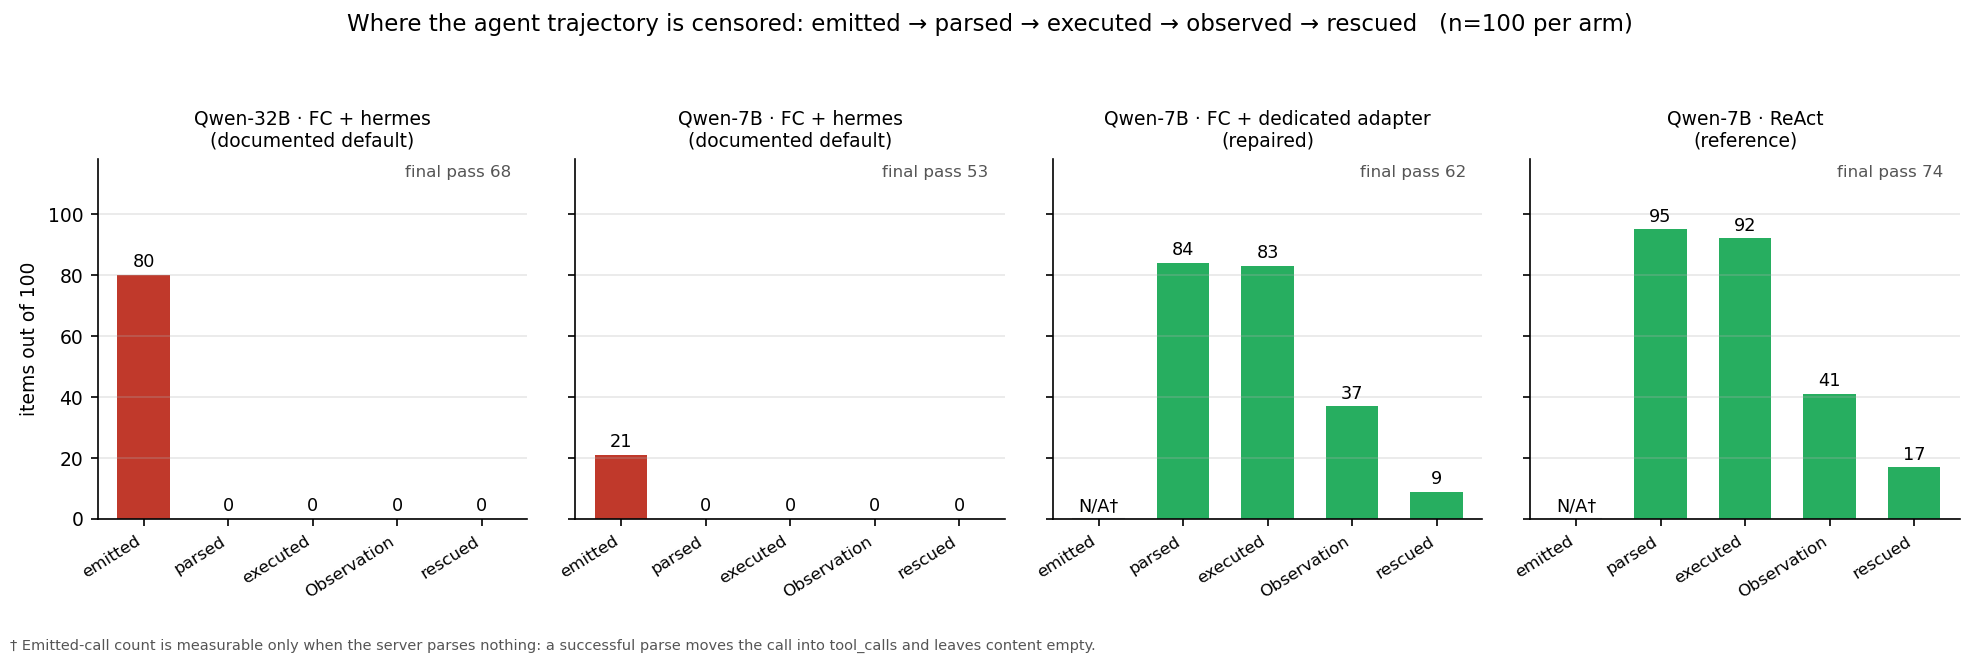
\includegraphics[width=\linewidth]{fig0_funnel.png}
\caption{\textbf{Where the agent trajectory is censored.} Five layers, $n{=}100$ per arm. The two
left panels (documented default configuration) show a tall first bar and a cliff to zero: the
model emits well-formed calls and nothing downstream happens. Emitted-call counts are measurable
only where the server parses nothing --- a successful parse moves the call into
\texttt{tool\_calls} and empties \texttt{content} --- so those cells are N/A, not zero.}
\label{fig:funnel}
\end{figure}

An agent evaluation does not measure a model. It measures a composition
\texttt{model $\times$ protocol $\times$ serialization $\times$ parser $\times$ execution stack},
and the failure of most stages is indistinguishable at the output from model incapability: when a
parser does not recognise the format a model emits, the serving layer reports zero tool calls ---
exactly what a model that refuses to use tools would produce. We call this
\textbf{interface-induced trajectory censoring}.\footnote{\emph{Censoring} is borrowed by analogy.
In survival analysis it is a threshold on a continuous variable; a parser is a deterministic
filter on output \emph{format}. What carries over is the structure of the inference error: the
observation is not missing at random, it is systematically unobservable on one side of a boundary,
and the boundary correlates with the quantity being measured --- positively with checkpoint size,
within this family.} It acts in two opposite directions, and our results contain a clean instance
of each: \textbf{masking}, where a valid call is not recognised and the action never reaches the
environment (Qwen2.5-Coder, \S\ref{sec:scale}), and \textbf{suppression}, where an invalid call is
removed from the sampleable support before it becomes an action (Llama-3.1-8B,
\S\ref{sec:llama}). The correct general statement is therefore neither ``the failure is in the
model'' nor ``the failure is in the interface'':

\begin{quote}
\textbf{The serving interface is simultaneously part of the measurement function and part of the
agent's effective action space.}
\end{quote}

Under RL this is literal. The interface sits between the policy and the environment: whatever the
policy emits must survive serialisation and parsing before it becomes an action that earns a
reward. When nothing tool-intended survives that passage, the experience distribution contains no
tool-mediated trajectory at all.

\paragraph{Why this is not a parser bug.}
The term invites a reading we refuse at the outset. Replaying vLLM's own \texttt{hermes} extractor
line by line over every stored first turn in our archive --- 4254 of them, after removing
byte-identical duplicate files --- we find zero cases in which the server failed to parse a call
its own rules would have accepted (\S\ref{sec:scale}). What fails is the \emph{contract} between
three parties configured independently: what the checkpoint was trained to emit, what the chat
template tells it to emit, and what the parser is defined to accept. Qwen2.5-Coder emits a
well-formed bare call and never the \texttt{<tool\_call>} envelope, so \texttt{hermes} not seeing
it is \emph{correct behaviour}; Qwen2.5-Instruct emits the envelope and then breaks the JSON
inside it. Censoring can occur at any boundary along
\texttt{emission $\to$ serialization $\to$ parse $\to$ execution}, and at every one the observable
is identical: HTTP 200 with an empty \texttt{tool\_calls} array. The claim is therefore not that
parsers are buggy but that \textbf{a tool-call rate is a property of a three-way contract, and is
routinely reported as though it were a property of the model alone.}

\paragraph{What is and is not new.}
That Qwen2.5-Coder does not emit \texttt{hermes}-format tool calls was reported in vLLM issue
\#32926 (2026-01-23) together with a \texttt{<tools>} parser proposal; it was closed as \emph{not
planned} and labelled \emph{stale}, so the trap is still live (\S\ref{sec:related}). What this
paper adds is measurement, decomposition and consequence. We measure the funnel on \emph{two}
standard benchmarks --- BFCL~v4 and $\tau$-bench --- where changing only the serving adapter moves
BFCL's reported score from 0.00 to 0.96 / 0.19 and $\tau$-bench's parsed calls from 0 to 636, and
a $2\times2$ over template and parser finds both main effects exactly zero with the whole effect
in their interaction (\S\ref{sec:bfcl}). We separate \emph{model intent} / \emph{emitted format} /
\emph{server parse} / \emph{actual execution} / \emph{multi-turn rescue} into five independently
measured quantities --- reporting only the third is the standard practice we argue against ---
quantify how much censoring removes across a 21$\times$ scale range, and pair that ladder with a
counterfactual under a \emph{matched} envelope where the silent fraction stays at 0--2 instead of
rising to 80 (\S\ref{sec:scale}). Four families failing at template, parser, schema and token
layers motivate a layered taxonomy, on deliberately asymmetric evidence we mark as such
(\S\ref{sec:families}). And we follow the distortion into training: at 7B, 45 of 115 generations
inside verl's AgentLoop carry a complete call and none becomes an action, so the sampled
experience contains no tool-mediated trajectory to reinforce. We argue that from the sampled
rollouts, not the support of the policy --- \emph{zero observed samples is not zero probability}
--- and the comparison arm changes protocol and interface together; the parser-repair control that
would separate them is a code change blocked by scale, not by the stack (\S\ref{sec:norepair}).
\label{end:01_intro}
\section{Related Work}

\textbf{Evaluation validity under nuisance factors.} A line of work shows that reported LLM
capability is sensitive to factors that ought to be irrelevant. \citet{sclar2024formatspread}~(\emph{FormatSpread})
quantify how prompt-formatting choices alone move benchmark scores by margins comparable to
model differences; \citet{mizrahi2024stateofwhatart}~(\emph{State of What Art?}) show single-prompt evaluation is
unreliable and argue for multi-prompt protocols; \citet{dehghani2021benchmarklottery}~(\emph{The Benchmark Lottery})
document how benchmark and configuration choices determine which method appears to win.
Our contribution is adjacent but distinct: those works vary an input the evaluator controls
and observe score movement. \textbf{We identify a component of the measurement apparatus --- the
serving stack's tool-call parser --- that can zero out a capability signal entirely, without
any error, and whose distortion grows with model scale.}

\textbf{Constrained decoding and its costs.} \citet{tam2024speakfreely}~(\emph{Let Me Speak Freely?}) report that
format restrictions and structured-output constraints can degrade reasoning. This bears
directly on \S5.3, where enabling \texttt{strict:\ true} eliminates a 23\% role-confusion failure and
\emph{improves} pass rate (49 $\to$ 61). We do not claim constraints are free: our result is that on
this task the constraint's benefit --- admitting 23 previously-discarded items into execution
--- outweighs any reasoning cost, and we report the CoT control (\S5.3) where added reasoning
made matters worse. Whether constraints hurt elsewhere in the same stack is untested here.
Guided-decoding machinery \citep{willard2023outlines} underlies both \texttt{strict} and vLLM's
\texttt{required} mode.

\textbf{Tool-use benchmarks.} BFCL~\citep{bfcl2025}, $\tau$-bench \citep{yao2025taubench}, ToolLLM~\citep{qin2024toolllm},
API-Bank~\citep{li2023apibank} and Toolformer~\citep{schick2023toolformer} evaluate or train tool use. To our
knowledge these report tool-call rates as parsed by the serving layer. \S5.2 shows that
number can be zero while 80/100 well-formed calls are emitted, which --- if the pattern
replicates on their stacks --- would affect any absolute tool-use rate they report.

\textbf{Protocols and agent loops.} ReAct~\citep{yao2023react} is the text protocol we compare against.
vLLM~\citep{kwon2023vllm} is the serving stack; its tool-calling documentation specifies distinct
per-family configuration, which \S5.1 shows is not optional. verl~\citep{sheng2025hybridflow} provides the RL training stack; importantly its AgentLoop performs \textbf{its own}
tool-call parsing (\texttt{verl/experimental/agent\_loop/tool\_parser.py}, adapted from vLLM v0.9.1),
so a vLLM-side parser plugin does not affect training rollouts --- a distinction that cost us
one wasted experiment design (\S5.6).

\textbf{Prior report of the Qwen case.} vLLM issue \#32926~\citep{vllm_issue_32926},
opened 2026-01-23, documents that Qwen2.5-Coder was not trained on tool-call tokens, that it
emits \texttt{json} fenced blocks or bare JSON absent format instructions, and that a
\texttt{<tools>} few-shot template plus a dedicated parser reaches 98--100\% compliance. The
issue was closed as \emph{not planned} and labelled \emph{stale}. Section~\ref{sec:scale}
reproduces this baseline exactly---zero \texttt{<tool\_call>} and \texttt{<tools>} tags at
every scale---and extends it to scale quantification, to three further families, and to
training. A related verl issue~\citep{verl_issue_4124} reports the same role-confusion
signature we characterise in Section~\ref{sec:llama}: the model calls the task function
(\texttt{solve\_equation}) and the agent loop raises \texttt{KeyError}.

\textbf{RL with tool feedback.} GRPO~\citep{shao2024deepseekmath} and RLOO~\citep{ahmadian2024rloo} are the estimators
we train with; EvalPlus~\citep{liu2023evalplus} and KodCode~\citep{kodcode2025} supply held-out evaluation and training
problems respectively. We are not aware of prior work measuring interface-layer censoring
of tool trajectories inside an RL rollout, nor connecting it to which capability the policy
gradient can reach.
\label{end:02_related}
\section{Setup}
\label{sec:setup}

\textbf{Task.} 100 problems drawn from a decontaminated KodCode subset (n-gram containment
against EvalPlus). \textbf{All 50 full-length arms in this paper use the identical 100 items}
(verified: unique item-set count = 1), so every cross-arm comparison is paired.

\textbf{Protocols.}
\emph{ReAct} --- a text protocol with \texttt{Thought:} / \texttt{Action:\ run\_tests} / \texttt{Action\ Input:\ \textasciigrave{}\textasciigrave{}\textasciigrave{}python\ \ldots{}\textasciigrave{}\textasciigrave{}\textasciigrave{}}
/ \texttt{Observation:}; the tool name is fixed in the template.
\emph{Function calling (FC)} --- OpenAI-style, \texttt{tool\_choice:\ auto}, one tool \texttt{run\_tests} taking a
single \texttt{code} string. Schema variants: \textbf{terse} (bare \texttt{\{"type":"string"\}}), \textbf{rich}
(parameter description, counter-example, code sample), \textbf{strict} (\texttt{strict:\ true},
\texttt{additionalProperties:\ false}).

\textbf{Serving.} vLLM 0.27.1~\citep{kwon2023vllm,vllm_toolcalling_docs}, per-family parser and chat template as documented.
\texttt{temperature=0} is greedy but \textbf{not bit-wise deterministic} under continuous batching:
identical prompts can differ across batch compositions. The main table is a single sample
per item; \S\ref{sec:variance} quantifies sampling variability separately at \texttt{temperature=0.6} rather than
assuming greedy decoding removes it.
\texttt{max\_tokens\ =\ 2048} for \textbf{both} protocols (see \texttt{ERRATA.md} \S\ref{sec:intro} --- an earlier asymmetry
favoured FC; re-running under the true shared limit changed final pass by $\leq$1 item).

\textbf{Measured quantities.} For each item's first turn we record: whether the server parsed a
tool call; the raw output; the tool name called; the raw \texttt{arguments}; \texttt{finish\_reason}; and
a protocol-agnostic intent classification (\S\ref{sec:intent}). Execution, per-turn results, and final
pass are recorded per turn.

\subsection{Intent criterion}
\label{sec:intent}

\emph{The criterion's source, the three tiers, and every
prompt and tool schema used in this paper are reproduced verbatim in Appendix~\ref{app:prompts}.}

Reporting only server-parsed calls is the practice under examination, so we need an
independent measure of what the model emitted. A single classifier (\texttt{analysis/intent.py})
is shared by all text, tables and figures:

\begin{itemize}
\tightlist
\item
  \textbf{tight} --- a JSON object naming \texttt{run\_tests} with an \texttt{arguments} object whose \texttt{code} is a
  \textbf{string literal containing real Python}. Excludes two contaminants we observed:

  \begin{enumerate}
  \def\labelenumi{(\roman{enumi})}
  \tightlist
  \item
    echoing the injected schema (\texttt{parameters}/\texttt{description} present, no \texttt{arguments});
  \item
    illustrative pseudo-code (\texttt{\{"code":\ test\_code\}} --- an identifier, not a string).
  \end{enumerate}
\item
  \textbf{strong} --- trajectory tag \texttt{json\_named\_call} or \texttt{xml\_tool\_call}.
\item
  \textbf{weak} --- JSON-shaped fragments only; at 1.5B these are almost entirely false positives
  and we report them separately rather than merging them.
\end{itemize}

\subsection{Human validation of the intent criterion}
\label{sec:humanval}

The scale trend in \S\ref{sec:scale} rests entirely on an automated classifier, so we validated it
against human judgement. 98 outputs were sampled \textbf{stratified by classifier verdict}
(40 \texttt{tight}, 28 \texttt{strong}-but-not-\texttt{tight}, 30 neither) --- deliberately over-sampling the
decision boundary so both false positives and false negatives are estimable. Sampling is
seeded and the annotator saw only the raw output, never the classifier's label.

We report \textbf{two rounds}, because the first one is itself a finding.

{\small
\begin{longtable}[]{@{}lllllll@{}}
\caption{Human validation of the intent criterion. Two annotation rounds on a stratified sample; round 2 supplied the model's own preceding turn as context. The classifier is used only to count what the server discarded, so its recall matters more than its precision --- and after correction it misses almost nothing.}\label{tab:validation}\\
\toprule
& agreement & Cohen's $\kappa$ & precision & recall & FP & FN \\
\midrule
\endfirsthead
\toprule
& agreement & Cohen's $\kappa$ & precision & recall & FP & FN \\
\midrule
\endhead
Round 1 (raw output only) & 86.7\% & 0.713 & 70.0\% & 96.6\% & 12 & 1 \\
After adjudication & \textbf{96.9\%} & \textbf{0.936} & \textbf{95.0\%} & 97.4\% & 2 & 1 \\
\bottomrule
\end{longtable}
}

The 12 round-1 false positives split into two causes, and the second one is ours, not the
annotator's. \textbf{Eleven are reading-order failures}: the tool call sits mid-document,
after a fenced \verb|```python| block (match positions 1209--2585 in outputs of median length
\textasciitilde2000); the annotator read the code block, concluded ``this is a direct answer,
not a call'', and stopped. \textbf{One is an instrument failure}: for a 32B item the matched
span begins at character 2585 and the annotation pack truncated every output at 2400, so the
evidence was \emph{not in the pack at all}. That item could not have been labelled correctly.
Re-shown the matched span alone, 10 of 13 disputed items were reversed.

We flag the second cause rather than folding it into the first because \textbf{the annotation
instrument reproduced the very failure this paper is about}: a truncating tool silently
removed the evidence, and what came out the other side was ``the model did not call the
tool''. The corrected pack (below) carries every output in full.

We report this rather than only the adjudicated figure because \textbf{it reproduces the paper's
mechanism on a human reader}: the evidence was present in every case, and what determined
whether it was seen was the order in which the text was scanned. The serving parser is
blocked by format; the annotator was blocked by reading order. Both produce the same
conclusion --- ``the model did not call the tool'' --- from the same bytes.

\textbf{The first adjudication was one-sided, and we do not treat its $\kappa$ as a reliability
estimate.} Auditing the procedure after the fact: the 13 adjudicated items were selected
\emph{exactly} as the items where the annotator disagreed with the classifier (13/13
overlap), and all 10 reversals moved \emph{toward} the classifier, none away. Under that
selection rule agreement can only rise, so $0.713 \to 0.936$ is a property of which items
were re-examined, not evidence of reliability. We report the second annotator instead.

\subsubsection*{A second independent annotator, and what it revealed about the first}

A second annotator, blind to the classifier, to the first annotator's labels and to the
first pack's item order, labelled the identical 98 items under a verbatim-identical rubric.
Two changes were made to the instrument: outputs are carried \textbf{in full} (the first
pack truncated at 2400 characters), and the adjudication rule was fixed in advance to review
\emph{all} three-way disagreements rather than only those disagreeing with the classifier.

\begin{table}[htbp]
\centering
\caption{Inter-annotator reliability. Restricting to items where both annotators read
identical bytes is not a convenience: 11 of the 12 raw disagreements are items the first
pack truncated, where A1 answered ``no call'' because the call had been cut from their copy.}
\label{tab:interannotator}
\small
\begin{tabular}{@{}lcc@{}}
\toprule
Cohen's $\kappa$ (95\% CI, bootstrap) & all items ($n$=97) & \textbf{identical bytes ($n$=62)} \\
\midrule
A1 vs.\ A2 (inter-annotator) & 0.736 [0.590, 0.863] & \textbf{0.967 [0.897, 1.000]} \\
A2 vs.\ classifier           & 0.936 [0.855, 1.000] & \textbf{0.967 [0.897, 1.000]} \\
A1 vs.\ classifier           & 0.712 [0.559, 0.847] & 0.934 [0.834, 1.000] \\
\bottomrule
\end{tabular}
\end{table}

\textbf{The apparent unreliability was the instrument, not the raters.} Of the 12 items where
the two annotators disagree, \textbf{11 are items whose full text exceeds 2400 characters},
and in every one of them A1 answered \texttt{N} while A2 answered \texttt{Y} --- A1 said ``no
call'' because the call was not in the copy they were given. On the 62 items where both read
identical bytes, the two annotators agree on 61 and \textbf{inter-annotator $\kappa$ = 0.967}.

We keep this rather than quietly regenerating a clean number, because it is the paper's own
thesis arriving uninvited in our methods section: \textbf{a truncating instrument sat between
the evidence and the observer, and what came out was ``the model did not call the tool''} ---
the same sentence the \texttt{hermes} parser produces, from the same bytes, for the same
reason. We were measuring censoring with a censored instrument.

\textbf{Third-party adjudication, and the final labels.} Fifteen items were not unanimous
across A1, A2 and the classifier. All fifteen went to a third adjudicator under the
pre-registered rule --- selected by \emph{any} three-way disagreement, never by disagreement
with the classifier --- who saw full text and no one else's labels. The adjudicator sided
with A2 on 11, with the classifier on 9, and with A1 on 6, and \textbf{moved away from the
classifier on 6 of 15}. That last number is the check that matters: the first round's
adjudication moved away from the classifier zero times out of thirteen, which is what an
outcome looks like when the selection rule has already decided it.

Combining the 83 unanimous items with the 15 adjudicated ones gives a gold standard that at
no point consulted the classifier.

\begin{table}[htbp]
\centering
\caption{Validation against the adjudicated gold standard. The inter-annotator column is
restricted to items where both annotators read identical bytes, because A1's pack truncated
at 2400 characters; the classifier and the gold standard are unaffected by that truncation
and are scored on the full sample.}
\label{tab:validation2}
\small
\begin{tabular}{@{}lcc@{}}
\toprule
Cohen's $\kappa$ (95\% CI, bootstrap) & full sample & identical bytes \\
 & ($n$=97) & ($n$=62) \\
\midrule
A1 vs.\ A2 (inter-annotator) & 0.736 [0.595, 0.866] & \textbf{0.967 [0.893, 1.000]} \\
Classifier vs.\ gold standard & \textbf{0.871 [0.756, 0.958]} & 0.934 [0.829, 1.000] \\
\bottomrule
\end{tabular}
\end{table}

\textbf{Correction factor.} Against the gold standard the \texttt{tight} stratum's precision
is 36/40 = \textbf{0.900}, so \S\ref{sec:scale}'s headline 80/100 at 32B corrects to \textbf{$\approx$72}.
The criterion errs in both directions --- 4 over-counts against 2 calls it misses entirely,
for a net over-count of 2 --- so the correction is smaller than the precision figure alone
suggests. \textbf{The trend is unaffected}: applying 0.900 uniformly gives
$0, 3.6, 18.9, 32.4, 72$ against a server-side zero at every size. We report uncorrected
classifier counts in all tables with this factor stated, rather than rescaling silently.

For the record, this number moved twice as the validation improved, and we report the
trajectory rather than only its endpoint: 0.950 under the first, one-sided adjudication;
0.975 under A2's labels alone; \textbf{0.900} against the adjudicated gold standard. The
first was inflated by its selection rule, the second rested on a single rater, and only the
third is built from a rule fixed before the labels were seen.

\textbf{A bound on the measurement itself.} The probe stores at most 4000 characters of raw
output per item; 10 of the 98 sampled outputs reach that ceiling, and one of the grey-zone
items above is a call truncated by it. The classifier and both annotators read identical
bytes, which is what agreement requires, but a call emitted beyond character 4000 is
invisible to all three. Emitted-call counts are accordingly a \textbf{lower bound} ---
conservative for our claim, since it can only understate the censoring we report.

\subsection{Validity gating}
\label{sec:gating}

An arm is admissible for pass-rate comparison only if it has exactly 100 items, exit code 0,
\textbf{zero request errors}, and provenance (model / protocol / temperature / \texttt{max\_tokens} /
adapter) matching the intended configuration. Arms with request errors retain a valid
\textbf{error-rate census} but are marked N/A for pass rates and \emph{no p-value is computed for
them}. This rule is enforced in code (\texttt{validate\_arms.py}, \texttt{final\_table.py}), not by
convention: an earlier draft computed \emph{p}=0.648 on such an arm, and that number is
retracted.

\begin{center}\rule{0.5\linewidth}{0.5pt}\end{center}
\label{end:03_setup}
\section{Positive Control: The Pipeline Works}
\label{sec:control}

Before attributing a zero to a model we verify the measuring instrument. On the \emph{same
live server}, same model, tools and system prompt, changing only \texttt{tool\_choice}:

{\footnotesize
\begin{verbatim}
tool_choice = auto      -> finish_reason = stop        tool_calls = 0
  content: "好的，下面是一个实现 count_distinct 的示例代码：```python..."
tool_choice = required  -> finish_reason = tool_calls  tool_calls = 1
  name = run_tests   arguments = {"code": "def count_distinct(nums): return len(set(nums))"}
\end{verbatim}
}

\noindent Under \texttt{required}, \texttt{hermes} parses correctly: server flag, parser and
chat template are all functional. \textbf{This establishes that the pipeline can accept a
conforming call; it does not by itself locate the zero under \texttt{auto} in the model},
because \texttt{required} uses constrained decoding and so says nothing about whether the
model spontaneously knows the \texttt{<tool\_call>} format. Separating the two requires the
emitted-intent measurement of \S\ref{sec:bfcl} onward. (Assistant content is reproduced
verbatim; our task prompts are in Chinese and we do not translate model output in
transcripts.)
\label{end:04_control}
\section{Results}
\label{sec:results}

Nine measurements, in the order the argument needs them. Each is stated here with its numbers;
the tables, the funnel columns behind them and the reproduction records are in
Appendix~\ref{app:extra}, and every scope condition is collected in \S\ref{sec:limitations}.

\subsection{BFCL v4: the score moves the whole span of the metric, and repair is complementary}
\label{sec:bfcl}

BFCL~v4 supplies official data, a multi-turn executor and a scorer at pinned Gorilla commit
\texttt{6ea57973c7a6097fd7c5915698c54c17c5b1b6c8}. Holding weights, cases, decoding, seeds,
executor and scorer fixed on 200 cases and changing \emph{only the serving adapter
configuration}, BFCL's own scorer reports \textbf{0.00} or \textbf{0.96 / 0.19}
(\texttt{simple\_python} / \texttt{multi\_turn\_base}) for the same model. The intervention is a
pair --- parser \emph{and} its chat template --- so we ran the $2\times2$ that separates them.

\begin{center}
\small
\captionof{table}{Template $\times$ parser on BFCL, first request per case.}\label{tab:bfcl2x2}
\begin{tabular}{@{}lll@{}}
\toprule
& documented template & dedicated template \\
\midrule
\texttt{hermes} parser & 0/200 & \textbf{0/200} \\
dedicated parser & \textbf{0/200} & 196/200 \\
\bottomrule
\end{tabular}
\end{center}

\textbf{Starting from the documented configuration, either one-component replacement recovers
0/200 calls, whereas replacing both components recovers 196/200.} These are simple effects at a
specified baseline, not zero marginal main effects. The $2\times2$ establishes strong
complementarity in parsing; BFCL scores were computed only for the two end-to-end corner
configurations, so the score swing itself is not decomposed over all four cells. Under the documented template the model writes a bare call inside a
\texttt{```json} fence; under the dedicated template it writes the same payload, byte for byte,
inside \texttt{<tools>} tags. Each parser behaves correctly for the envelope it is defined to
accept, so no component is defective and repairing one side of the contract buys exactly nothing.
The funnel behind those scores: the documented arm parses \textbf{0 of 200} first requests with
zero HTTP errors, while \textbf{166} of those same responses carry a call meeting the strict
criterion; the repaired arm parses 196, executes 98 of 100 \texttt{multi\_turn\_base} cases and
succeeds on \textbf{19}, against 0 executed and 0 succeeded for \texttt{hermes}, whose zero is
therefore \emph{by construction rather than by capability}
(Tables~\ref{tab:bfclfunnel}--\ref{tab:bfcl5}). \textbf{A published benchmark number for this
model can differ by the entire span of the metric depending on a serving flag the model card does
not mention.} We claim only that 0.00 is not a measurement of the model; and since the repaired
arm uses the community adapter, not a verified-optimal one, and still fails 4 of 200. We therefore
report $0\to19$ as the recovery achieved by this adapter, not as an estimate of an optimal model
or interface score.

BFCL's shipped handler for local Qwen models bypasses the serving parser entirely, so we route
BFCL's own OpenAI handler through \texttt{/v1/chat/completions}, adding only
\texttt{tool\_choice: auto} and trace headers; dataset loading, execution and scoring remain
BFCL's code and \texttt{bfcl\_eval}'s files are byte-identical (Appendix~\ref{app:bfcl}).

\subsection{$\tau$-bench: the mechanism survives a simulated user and a stateful environment}
\label{sec:tau}

BFCL scores a single trajectory against a final state. $\tau$-bench \citep{yao2025taubench} adds a
simulated user and a stateful environment, so a censored call costs not one action but the rest of
the conversation. Across all 115 \texttt{retail} tasks, paired across arms with none dropped and
changing only the serving adapter: server-parsed calls \textbf{0 versus 636}, tool executions
\textbf{0 versus 636}, and tasks reaching \emph{any} tool execution \textbf{0 versus 103}. Every
one of the documented arm's 1389 requests carried \texttt{tools}, not one was parsed, and 789
assistant turns carried a call-shaped payload the server discarded (Table~\ref{tab:tau}).
\textbf{The task-outcome difference does not reach significance and we do not claim it}: 7 versus
10 solved, three discordant pairs all in the repaired direction, exact McNemar \emph{p}=0.25, with
the documented arm's solved set a strict subset of the repaired arm's. Two scope conditions belong
with these numbers rather than in a footnote: the user simulator is a locally served
Llama-3.1-8B rather than the \texttt{gpt-4o} of the original harness, so \textbf{the absolute
scores are not comparable to the $\tau$-bench leaderboard} and only the between-arm difference is
claimed; and the arms differ in conversation length by construction, which is why every quantity
is per task and not per request.

\paragraph{The envelope layer is domain-invariant; the payload layer is not.}
$\tau$-bench also lets us ask whether the \emph{failure layer} travels across domains, because
its arguments are short scalars (\texttt{\{"order\_id": "W123"\}}) where our own task passes a
whole program as a string. Replaying vLLM's extractor over the documented arm's 789
emitted-but-unparsed assistant turns puts \textbf{789 of 789 (100\%) at the envelope layer}, with
\textbf{0} malformed payloads, \textbf{0} recoverable by lenient decoding, and --- as everywhere
else in this paper --- \textbf{0 genuine parser losses}. The emissions carry the same signature as
the code task: a bare call inside a \texttt{```json} fence, never the \texttt{<tool\_call>}
envelope. This matters in two directions. The layer that carries our headline result is
\textbf{unchanged by the domain}, and the running total of first turns in which the server
discarded a call its own extractor would have accepted stays at zero across code and non-code
alike. But the \emph{other} layer moves: Qwen2.5-Instruct loses 41\% of its unparsed items to
malformed payloads on the code task (Table~\ref{tab:layer}), almost always by leaving docstring
quotes or raw newlines unescaped inside a \texttt{code} string --- a failure mode that short
scalar arguments cannot produce. \textbf{We therefore expect the envelope-layer result to
generalise and the payload-layer proportions not to}, and we state that as a prediction rather
than a measurement, having tested one non-code domain and not a sample of them.

\subsection{Censoring against scale, and the same scale under a matched interface}
\label{sec:scale}

Our own probe, across the Qwen2.5-Coder ladder under \texttt{tool\_choice: auto} and
\texttt{hermes} --- the documented recommendation for Qwen2.5 --- n=100 per size.

\begin{center}
\small
\captionof{table}{Qwen2.5-Coder under the documented \texttt{hermes} configuration, n=100 per size.}\label{tab:scale}
\begin{tabular}{@{}llllll@{}}
\toprule
Size & Server-parsed & \textbf{tight} & strong ($\supseteq$ tight) & weak (disjoint) & Final pass \\
\midrule
1.5B & 0 & 0 & 0 & 27* & 31 \\
3B & 0 & 4 & 5 & 28 & 37 \\
7B & 0 & 21 & 22 & 1 & 53 \\
14B & 0 & 36 & 42 & 3 & 53 \\
\textbf{32B} & \textbf{0} & \textbf{80} & 100 & 0 & 68 \\
\bottomrule
\end{tabular}
\end{center}

Across a 21$\times$ range the server reports a flat zero while well-formed emitted calls rise to
80/100 ($\approx$72 after the 0.900 correction factor of \S\ref{sec:humanval}, assuming
tight-stratum precision transfers across sizes).
\textbf{Within this family, the larger the checkpoint, the larger the absolute undercount under
the same mismatched interface} --- a within-family observation across five checkpoints, not a law
relating capability to censoring. Raw-tag counts reproduce vLLM issue \#32926's baseline exactly:
\texttt{<tool\_call>} and \texttt{<tools>} appear zero times at every size. Two offline analyses
close the obvious objections (Appendix~\ref{app:reparse}): re-parsing the \emph{same stored bytes}
under four rules excludes ``your extractor is simply better than \texttt{hermes}'', and replaying
vLLM's extractor line for line to locate each loss shows \textbf{genuine parser loss is zero in
every arm}, across all 4254 de-duplicated first turns.\footnote{The 1.5B row uses the
\emph{optional} tool instruction; under the \emph{mandatory} prompt used for training
(\S\ref{sec:rl}) the same checkpoint gives weak = 66 and unparsable = 46. Coercion produces more
JSON-shaped debris, not more valid calls.}

\paragraph{A matched-interface supporting ladder through 8B.} The server column is flat zero, so the growth comes entirely from
the emitted column --- and larger checkpoints emit more well-formed JSON for reasons unrelated to
tool calling. Qwen3 supplies a ladder whose template injects tools and requires the
\texttt{<tool\_call>} envelope \texttt{hermes} accepts; the prediction (``parsed $>0$ at every
size'') was committed to the repository before running (\texttt{p4/PREREGISTRATION.md}).
Server-parsed counts are 86 / 44 / 70 / 97 at 0.6B--8B, and the silent fraction through 8B is
\textbf{1, 1, 2, 0} against the mismatched ladder's 0, 4, 21, 36, 80
(Table~\ref{tab:counterfactual}). \textbf{Across a comparable span of scale under a matched
envelope, we do not observe the growing silent fraction seen in Qwen2.5-Coder.} This is a
cross-family supporting observation, not a strict scale counterfactual: it changes family and
envelope together and does not independently measure capability growth. Two caveats we state rather than bury: the parsed column is \textbf{not
monotone}, so this shows presence, not a trend; and Qwen3 was served with
\texttt{enable\_thinking=false}, because with thinking on the model exhausts its token budget in a
\texttt{<think>} block before emitting a call --- a confound unrelated to the envelope, recorded
as a protocol deviation before the run.

A second family showing the \emph{same} undercount would be stronger, and we did not get one. Of
nine families surveyed beforehand, six do not inject OpenAI-style tools at all; of the remaining
three, Granite-3.1-8B does not attempt tool calls on this task --- 0 under \texttt{hermes}
\emph{and} 0 under its own \texttt{granite} parser. \textbf{That rescue arm is what tells us the
arm is uninformative rather than confirmatory}, and we claim nothing from it.

\subsection{Within-lineage control, and the ceiling it puts on multi-turn rescue}
\label{sec:instruct}

Changing family cannot test the scale result --- Llama parses correctly, Mistral returns 400,
DeepSeek never injects the template, so none can exhibit censoring at all.
Qwen2.5-\textbf{Instruct} can: it shares Coder's chat template, which is what produces the
false-positive template check of \S\ref{sec:families}, and differs in whether the checkpoint was
trained on tool-call tokens. On the same items, parser, \texttt{tool\_choice}, temperature and
seed, its server-parsed rate runs \textbf{1, 11, 63, 77, 88} against Coder's flat zero
(Table~\ref{tab:turn1}). \textbf{The contrast localises the mismatch to checkpoint-specific
training rather than to the shared family and template, or to parameter count alone.} We stop
short of naming tool-call-format training as \emph{the} cause: the two differ in their whole
post-training mixture, and this varies the bundle, not one element. It also answers the objection
that Instruct emits better-shaped calls around worse contents --- it solves 13--42\% of items on
turn~1 and 13--65\% by the end, nowhere near the zero that would require.

The multi-turn layer was initially void, because that host lacked \texttt{pytest}; we re-ran all
five arms with the executor working, changing nothing else and not touching the probe binary, and
the parsed column reproduced value for value. \textbf{Rescues then rise with the parsed column} ---
0, +3, +6, +14, +23 against 1, 11, 63, 77, 88, monotone together. Coder's first-turn and final
passes are identical at every size (31/31, 37/37, 53/53, 53/53, 68/68), which it would be natural
to read as multi-turn repair being useless at this scale; the Instruct ladder, on the same items
and criterion, shows it is not. We therefore state the repair result as a ceiling rather than an
absence: \textbf{how much multi-turn recovers is bounded by how much of the tool channel the
interface leaves open.}

\subsection{A 23\% failure that survived three controls and fell to the fourth}
\label{sec:llama}

Llama-3.1-8B under FC issues a tool call on 97/100 items, but on 23 the call names \emph{the
function the task asks it to implement}, with that function's own parameters as arguments; a re-run
restricted to those 23 reproduced 23/23. \emph{This also corrects a measurement of our own}:
because the probe did not verify the tool name, these 23 were counted as initiations, so
\textbf{Llama's true \texttt{run\_tests} initiation rate is 74/100, not 97/100}
(Appendix~\ref{app:errata}). Four single-variable paired controls: a richer schema explicitly
warning that the tool is not the task function left it at 22/100 (\emph{p}=1.000); a Thought
scaffold before the call raised it to \textbf{59} (\emph{p}\textless0.001, \emph{worse}), the model
supplying exactly the parameters it had just reasoned about; the official chat template moved
nothing (23$\to$22, wrong-tool discordances 1/0, exact \emph{p}=1.000); \texttt{strict: true}
on the official-template baseline took it from 22 to \textbf{0} (22/0, exact
\emph{p}=4.77$\times10^{-7}$). The earlier 0.125 and 0.0001 labels came from different outcome
comparisons and are withdrawn from the wrong-tool table. The first three rejected their alternative explanations and pointed at the
model; the fourth found the cause and withdrew that conclusion.

Adding \texttt{strict} to the official-template arm drives wrong-tool calls from 22 to 0, valid
execution from 73 to 97, turn-1 pass from 33 to 46, and final pass from 44 to 61. Thus the
single-variable final change is +17 (Table~\ref{tab:llama_arms}). The ReAct decomposition instead
uses terse FC (49) as its baseline and official-template-plus-strict (61) as the repaired endpoint,
so its broader interface-bundle contribution is \textbf{+12} (\emph{p}=0.0075), followed by
\textbf{protocol, +19}
(\emph{p}=0.0019), against +31 for both (Table~\ref{tab:decomposition}) --- \textbf{roughly two
fifths of what looked like a protocol effect was an interface effect}. With \texttt{strict} the two
protocols have identical execution mechanics (98 calls, 0 wrong-tool, 97 executed on both sides)
yet turn-1 differs 46 vs 61, so what remains is first-draft code quality under the protocol, not
tool-use mechanics. The defensible statement is narrower than either ``model defect'' or
``configuration bug'': \textbf{the model exhibits role confusion under unconstrained function
calling, and the interface constraint determines whether that confusion can be expressed as an
environment action.} We cannot show the tendency disappears once constrained, only that it stops
reaching the action space.

\subsection{Four layers, and what a pre-flight check can see}
\label{sec:taxonomy}
\label{sec:families}

The two families above fail at different layers with different remedies --- Qwen2.5-Coder at the
\emph{parser} layer, repaired by a dedicated adapter; Llama at the \emph{schema} layer, repaired by
\texttt{strict: true} --- and neither is caught by the obvious pre-flight test. Two further
families extend the taxonomy without supporting a quantitative comparison, and we report them as
such. \textbf{DeepSeek-Coder} fails at the \emph{template} layer: its chat template never injects
tools, which a template check does catch, and we found no remedy. \textbf{Mistral-7B-v0.3} fails at
the \emph{token} layer, repeating a \texttt{[TOOL\_CALLS]} marker that produces HTTP 400, and has
\textbf{no admissible 100-item FC run at all} --- all four configurations produce request errors
(parser only 2; official template 42; parser + strict 3; official template + strict 39), so vLLM's
own recommended configuration \emph{raises} the error rate from 2\% to 42\% and \texttt{strict},
which fixes Llama, does not help (Table~\ref{tab:taxonomy}).

Mistral is the one family whose failure announces itself; the other three return HTTP 200 with
\texttt{tool\_calls: []}, byte-identical to a model that declined to call the tool. \textbf{The
claim is not that all failures are silent; it is that the silent ones dominate and are the hardest
to attribute.} The natural pre-flight test --- does \texttt{apply\_chat\_template(tools=...)}
render the schema? --- correctly rejects DeepSeek-Coder but \emph{passes} Qwen2.5-Coder, which
inherits Hermes scaffolding from Qwen2.5-Instruct while never having been trained on it:
\textbf{protocol support is a per-checkpoint property and is not inferable from the chat
template.}

\subsection{Repair loop: how much comes back}
\label{sec:repair}
\label{sec:maintable}

On Qwen2.5-Coder-7B with \texttt{tool\_choice: auto} held fixed and only the adapter changed,
parse goes \textbf{0$\to$84}, items reaching a second turn \textbf{0$\to$37} and multi-turn rescues
\textbf{0$\to$9}: the mechanism is restored from literal zero (Table~\ref{tab:repair}). The two FC
arms have identical aggregate turn-1 pass, 53 vs 53. Because the evaluation adapter changes
parser, template and few-shot together, equality of this aggregate does not establish identical
first-turn generations and cannot by itself locate the failure layer. Llama's generation-time
constraint does move turn-1 pass (34$\to$46), but we use fixed-output replay and per-event tracing,
not the direction of aggregate score movement, to localize both mechanisms.

The pass-rate gain is \emph{not} significant (53$\to$62, \emph{p}=0.093). A pre-planned replication
on a random 300-item sample reproduces the direction (160/300$\to$178/300, 43 discordant against
25, \emph{p}=0.0385) --- nominally below 0.05, but this paper runs roughly a dozen McNemar tests
and the Bonferroni threshold is $\approx$0.0042, so \textbf{the repair gain still does not survive
correction and we rest no claim on it.} The protocol gap on the same 300 items
(178/300$\to$219/300, \emph{p}=3.1$\times$10$^{-6}$) clears it by three orders of magnitude.
Restricting to items both arms parsed, the residual protocol gap holds on Llama (\emph{p}=0.0021)
and is not detected on Qwen: $+8.4$\,pp, 95\% CI $[-0.5,+17.4]$, \emph{p}=0.118. \textbf{We do not
read $p>0.05$ as evidence of no effect} --- that interval admits a residual larger than the effect
we detect on Llama --- so the residual is established on one family and undetermined on the other
(Appendix~\ref{app:conditioned}).

\subsection{Parser repair restores RL experience; no held-out improvement detected}
\label{sec:rl}
\label{sec:norepair}
\label{sec:sufficiency}

The historical 1.5B result is over-determined: zero calls executed, but a replication under the
same mandatory prompt finds no well-formed call naming \texttt{run\_tests}. At 7B, by contrast, a
probe inside verl's AgentLoop records 45 complete bare-JSON calls in 115 generations, of which
\texttt{hermes} accepts none; its actor update then OOMs, so that
probe establishes the failure layer but not a learning effect. We therefore ran the missing
control: two preregistered 150-step GRPO arms at 7B under identical LoRA configuration, data,
prompt, seed, decoding, verifier and evaluation. The sole intervention is
\texttt{multi\_turn.format}: verl's stock \texttt{hermes} parser versus a registered parser that
accepts Qwen2.5-Coder's emitted format. Full rollout text, parser verdicts, executions and returned
observations were retained.

\begin{center}
\small
\captionof{table}{Formal 7B RL control. Event counts exclude held-out evaluation; outcome counts use the paired 542-item multi-turn split.}\label{tab:p3formal}
\begin{tabular}{@{}lrrrrr@{}}
\toprule
arm & tight emissions & accepted & executed/observed & final, step 0$\to$150 & rescues, 0$\to$150 \\
\midrule
broken FC & 8{,}689 & 10 & 10 & 430$\to$430 & 12$\to$12 \\
repaired FC & 17{,}608 & 16{,}912 & 16{,}844 & 430$\to$427 & 12$\to$12 \\
\bottomrule
\end{tabular}
\end{center}

The 16{,}912 accepted calls occur in 16{,}844 assistant-generation events: 40 generations contain
multiple calls and contribute 68 calls beyond the first. The AgentLoop dispatches one event per
generation; all 16{,}844 dispatches execute and return an observation. The tight classifier and
parser acceptance are not nested sets, so their marginal totals should not be read as a sequential
drop of 696 calls; Appendix~\ref{app:p3curve} gives the event-level cross-tabulation.

The broken channel is therefore \emph{nearly}, not literally, closed: only 10 of 8{,}689
tight-classified call emissions become actions. Parser repair changes the sampled experience by
more than three orders
of magnitude and returns an observation for every executed call, while holding the learning
problem fixed. This is direct causal evidence that the interface determines which emitted
behaviour enters RL experience; it supersedes the earlier, confounded ReAct comparison for that
claim.

It does not yield an outcome gain. Repaired FC ends at 415/542 turn-1 passes and 427/542 final
passes, versus 418/542 and 430/542 for broken FC; all three missing final passes are discordant in
the repaired-to-broken direction (paired difference $-0.55$ percentage points; approximate paired
95\% CI $[-1.18,0.07]$; exact McNemar $p=0.25$). Relative to its own step 0, repaired FC
has one gain and four losses ($p=0.375$), and multi-turn rescues remain exactly 12. We do not read
either non-significant difference as harm. \textbf{At this model scale, 150-step budget and single
seed, repairing the parser restores tool-mediated experience, but we detect no improvement in
held-out success or rescue counts.} The earlier 75-step ReAct arm points in the
same direction but is now only supporting evidence, because it changes protocol as well as
interface.

Both arms use LoRA rank 32 because 7B full-parameter RL does not fit a single 80\,GB card. The
held-out evaluation is identical across arms and bypasses both training parsers: verl's native
rollout RPC queries the current LoRA at temperature 0 for up to four 1,024-token
programmatic-feedback turns on the same 542 EvalPlus items, then appends sandboxed test output as
a user message. Each request attests the loaded global weight step, explaining why the
broken-training arm can still exhibit 12 evaluation rescues. The repaired process was interrupted
after step 116 and resumed from the step-90 checkpoint; before
resumption we verified model, optimizer, scheduler, RNG and dataloader state, source and
configuration hashes, and native checkpoint weight steps. The repeated step-90 evaluation differs
by two final-pass items (428 versus 426), which we report as test--retest variation; the formal
curve uses the original step-90 result and the weight-attested resumed step-120/150 results.
Mechanism totals combine original steps 1--90 with resumed steps 91--150 and exclude the abandoned
26-update step-91--116 branch. Appendix~\ref{app:p3curve} reports every checkpoint, training-log
diagnostics, checkpoint tensor deltas, and the machine-verifiable final-lineage manifest.
\label{end:05_results}
\section{Discussion}
\label{sec:discussion}

\textbf{Report the composition, not the model.} Any claim of the form ``model \emph{M} does not
use tools'' is, as measured, a claim about
\texttt{M $\times$ protocol $\times$ serialization $\times$ parser $\times$ stack}. Agent
evaluations should report at minimum (i) server-parsed calls, (ii) emitted-but-unparsed calls
under a stated criterion, (iii) request errors, and (iv) the exact serving configuration.
Reporting only (i) is the practice this paper argues against, and (ii) is where the 21$\times$
scale trend lives.

\textbf{Pre-flight, don't post-hoc.} A missing \texttt{-\/-enable-auto-tool-choice} is the only
failure that announces itself, and template inspection alone is insufficient
(\S\ref{sec:families}). We therefore treat a \texttt{tools}-bearing request returning HTTP 200 ---
\emph{and} a server-parsed call under \texttt{tool\_choice: required} --- as a required pre-flight
for any FC experiment, shipped as a 98-line script (\texttt{preflight\_toolcall.py}) that issues
one canonical request, asserts \texttt{tool\_calls} is non-empty with the expected \texttt{name}
and parseable \texttt{arguments}, then repeats under \texttt{required} as a positive control. It
runs in seconds and would have caught every silent failure in this paper.

\textbf{The guidance for this flag lives in the wrong place.} We surveyed the HuggingFace model
cards of nine families for any mention of \texttt{-\/-tool-call-parser}. Of the eight reachable
cards, none mentions it, while six recommend serving the model with vLLM. The publisher tells you
which server to use, the server asks you which parser to use, and neither treats the pairing as
its responsibility. We do \emph{not} read this as evidence that mismatch is common in deployment
--- we surveyed documents, not deployments, and vLLM ships dedicated parsers for some forty
families, so following \emph{its} table generally works. The claim is narrower: \textbf{the one
piece of configuration that can silently zero a capability measurement is documented by neither
party at the point of use.}

\textbf{Interface repair precedes protocol comparison.} On Llama the ReAct-vs-FC gap was 31 points
before the \texttt{strict} fix and 19 after, both components separately significant. On Qwen,
conditioning on parsed items, we do not detect a residual (\emph{p}=0.118) --- but that interval is
wide enough to contain effects as large as the unconditioned gap, so it is evidence of
\emph{insufficient resolution}, not equivalence. \textbf{Comparisons of agent protocols that do not
first exhaust the serving configuration matrix are not measuring protocols.}

\textbf{A cold-start hazard for agentic RL.} In the formal control, the mismatched parser admits
only 10 executions from 8{,}689 tight-classified call-like emissions while a tool-free reward path remains open;
the repaired parser admits 16{,}844 executed tool interactions. This isolates access to sampled tool
experience from learning from that experience: the first changes by more than three orders of magnitude,
while held-out rescues do not change. Practitioners should therefore verify both a
\textbf{non-trivial tool-execution count in the first training step} and a held-out measure of the
behaviour the tool is meant to teach. A rising reward curve establishes neither by itself.
\label{end:06_discussion}
\section{Limitations}
\label{sec:limitations}

Seventeen limitations, in the order a sceptical reader should apply them, are stated in full in
Appendix~\ref{app:limitations}; the six that most constrain what may be concluded are here.

\textbf{The scale result is within one family.} The $0\to4\to21\to36\to80$ ladder is
Qwen2.5-Coder alone, against one mismatched interface, on one task (item~3). We claim a
within-family monotone relation between checkpoint size and absolute undercount; we do not claim
censoring is generally scale-increasing, and we do not equate parameter count with capability. A
second \emph{family}'s ladder is the test that would promote or refute it.

\textbf{The repaired-FC control is one seed at one budget} (item~8). It is a clean parser-registry
intervention at 7B, but both arms use LoRA and 150 steps on one code task. It establishes the
experience-distribution effect in this setting; its null learning result is not a theorem that a
working channel can never help, nor is it strictly comparable to the historical 1.5B
full-parameter runs.

\textbf{Near-zero samples are not zero policy probability} (items~10--11). The broken 7B arm
retains full rollout text and distinguishes 8{,}689 tight-classified call emissions from 10 accepted and
executed calls, so attempts and discards are directly separated there. The older 1.5B run did not
retain full text and remains over-determined; neither run identifies the support of the policy
beyond its sampled trajectories.

\textbf{Conditioning on a successful parse is post-treatment conditioning} (item~9). Whether an
item parses is determined by the interface under test, so the both-parsed subset is not a random
subsample. On Qwen the residual is $+8.4$\,pp, 95\% CI $[-0.5,+17.4]$, $p$=0.118: \textbf{we do
not detect a residual difference, which is not the same as establishing there is none.}

\textbf{Multiple comparisons} (item~6). Roughly a dozen McNemar tests; the Bonferroni threshold is
$\approx$0.0042. Surviving it: the official-template \texttt{strict: true} intervention on
wrong-tool labels ($p=4.77\times10^{-7}$), its final-pass contrast ($p=7.63\times10^{-5}$), and the
protocol gap on 300 random items ($p$=3.1$\times$10$^{-6}$). \textbf{Not surviving it}: the
repair-loop pass gain ($p$=0.093 at $n$=100, $p$=0.0385 at $n$=300), the Llama protocol contrast
at $n$=300 ($p$=0.0352), the $\tau$-bench outcome difference ($p$=0.25), and the residual-gap
estimates ($p$=0.118, 0.125). We rest no claim on the latter group.

\textbf{The historical training verifier had two exploitable seams} (item~14): an unanchored
\texttt{passed} regex and a denominator omitting skipped/expected-failure tests. We audited the
historical logs; before the formal 7B control we also anchored the regex, counted all pytest
outcomes, and retained complete rollout text with hashes. Both P3 arms use that same repaired
verifier, so verifier changes cannot explain their contrast; the older learning curves remain
supported by an audit rather than a rerun.

Also constraining, and stated in full in the appendix: one task family and one tool (item~1); a
non-random 100-item set, whose 7B rung the random 300-item replication moves from 21 to 30
(item~2); a deliberately asymmetric taxonomy in which Mistral has no admissible FC comparison at
all (item~4); single-sample headline arms (item~5); scale stopping at 32B (item~7); sufficiency
tested by one repaired-FC seed and budget (item~12); a stratified validation sample with a 4000-character output
cap that creates false negatives while classifier imprecision creates false positives, leaving
the raw count's net bias unidentified (item~13); dependence on vLLM 0.27.1, verl 0.9.0
and publisher-mutable chat templates (items~15--16); and the instrumentation errata we disclose
rather than absorb --- seven arms recording \texttt{max\_tokens} they did not run at, Llama's
initiation rate corrected from 97 to 74, and one previously reported $p$=0.648 withdrawn
(item~17, Appendix~\ref{app:errata}).

\subsection*{What would change our conclusions}
\label{sec:future}

We name these so the claims are falsifiable rather than merely hedged.
\emph{Replications or a longer repaired-FC budget.} The completed single-variable control restores
16{,}844 tool interactions without moving held-out rescues. A consistent rescue gain over
additional seeds or a longer preregistered horizon would narrow the scope of this 150-step,
single-seed observation; continued nulls would strengthen it within, but not beyond, the tested
model/task setting.
\emph{A second family's scale ladder}, with a working test executor: if the undercount does not
grow with checkpoint size elsewhere, \S\ref{sec:scale}'s claim is a Qwen-plus-\texttt{hermes} fact
rather than a scaling phenomenon.
\emph{The same ladder on a non-code task.} The five Qwen2.5-Coder checkpoints run against
$\tau$-bench \texttt{retail} under the documented configuration --- models and interface fixed,
only the domain varied. If the emitted column still rises with size while the parsed column stays
at zero, the scale result is a property of the interface; if it does not, it is a property of
code-shaped payloads. This needs a rescue arm at the small sizes for the reason Granite did: a
checkpoint that simply never attempts a call produces an uninformative zero, not a censored one.
\emph{The same five-layer measurement on further benchmarks.} Done for BFCL~v4 and $\tau$-bench
\texttt{retail}, so the concern is not specific to our harness and now covers one interactive
suite; suites with much larger tool schemas, or whose scoring depends on argument-level matching,
remain untested.
\label{end:07_limitations}
\section{Conclusion}

Tool-call interfaces censor agent trajectories, silently and per checkpoint; within Qwen2.5-Coder
the absolute undercount rises monotonically with checkpoint size, which we report as a
within-family observation rather than a general law. In a 150-step RL control differing only in
verl's parser registry, the mismatched arm turns 8{,}689 tight-classified call-like emissions into 10 executions,
whereas the repaired arm executes and observes 16{,}844 calls. The intervention therefore restores
the tool-mediated experience distribution. We detect no held-out improvement: rescues remain 12
and final passes move from 430/542 to 427/542. Access to a trajectory and learning from it are
separate empirical questions.

Two controls fix what the effect is a property of. A $2\times2$ over chat template and parser on a
public benchmark finds zero recovery from either one-component replacement at the documented
baseline and 196/200 parses under joint replacement; and a supporting ladder under a
\emph{matched} interface holds the silent fraction at 0--2 across
a comparable span of scale, where the mismatched interface takes it to 80. \textbf{What the serving
layer removes is not a property of the model, nor of the parser, but of the contract between them.}

The most uncomfortable finding is methodological. We ran three single-variable paired controls on a
23\% failure and concluded it was a model deficiency; a fourth, taken from a sentence in the serving
documentation, reduced it to zero. Our own human validation reproduced the same mechanism: twelve of
ninety-eight annotations missed a tool call because it sat after a fenced code block, and the
annotator --- like the parser --- concluded from the same bytes that no call had been made.
Reporting server-parsed tool-call rates as model capability is not a safe default.
\label{end:08_conclusion}

\label{endofbody}
\bibliographystyle{plainnat}
\bibliography{refs}

\appendix
\section{Data Errata}

\emph{Every number in this paper traces to a trajectory file under
\texttt{runs/final/}. This appendix lists the files whose recorded provenance is wrong, the
arms that are inadmissible for pass-rate comparison, and what was verified correct. It is
reproduced from \texttt{runs/final/ERRATA.md} in the released repository.}

\subsection{Seven ReAct arms record the wrong \texttt{max\_tokens}}

The following files record \texttt{max\_tokens=2048} while the generation limit in force
was \textbf{1024}. Cause: \texttt{gen()} in the probe carried a default of
\texttt{max\_tokens=1024} while \texttt{gen\_fc()} used the global \texttt{MAX\_TOKENS=2048},
and the provenance written to disk recorded \texttt{MAX\_TOKENS} for both. Fixed
2026-08-31.

{\footnotesize
\begin{verbatim}
traj_v3_Llama8B_react.jsonl        recorded 2048 / actual 1024
traj_v3_Qwen7B_react.jsonl         recorded 2048 / actual 1024
traj_v3_Mistral7B_react.jsonl      recorded 2048 / actual 1024
traj_v11_DS1.3b_react.jsonl        recorded 2048 / actual 1024
traj_v11_DS6.7b_react.jsonl        recorded 2048 / actual 1024
traj_v11_Llama32_1B_react.jsonl    recorded 2048 / actual 1024
traj_v11_Llama32_3B_react.jsonl    recorded 2048 / actual 1024
\end{verbatim}
}

\textbf{Direction of the bias.} The contemporaneous FC arms were genuinely at 2048, so in
every affected ReAct-vs-FC comparison \textbf{the function-calling side had the larger
generation budget}. ReAct nonetheless won those comparisons, so the reported protocol gaps
are \emph{conservative}; correcting the asymmetry can only widen them. Re-running the three
main ReAct arms at a true 2048 changed final pass by at most one item
($80\to80$, $74\to74$, $32\to33$), which is why the correction is small in practice.

\textbf{Replacement data.} The four v11 arms are superseded by
\texttt{traj\_v13\_*\_react.jsonl}; the three v3 arms by \texttt{traj\_v14\_*\_react.jsonl}.
All tables in this paper cite the v13/v14 versions; the v3/v11 ReAct arms are retained only
as a record.

\subsection{Llama-3.1-8B initiation rate required manual correction}

\texttt{traj\_v3\_Llama8B\_fc.jsonl} records an initiation rate of 97/100, but 23 of those
calls target \textbf{the task function rather than \texttt{run\_tests}}. The probe did not
verify tool names when that batch was collected, so \texttt{has\_action} did not distinguish
them. \textbf{The corrected \texttt{run\_tests} initiation rate is 74/100.}

A re-run restricted to exactly those 23 items under matched configuration
(\texttt{traj\_v8\_Llama8B\_recheck.jsonl}, seed fixed) reproduced 23/23 as wrong-tool
calls, with names such as \texttt{can\_form\_word}, \texttt{check\_password\_strength} and
\texttt{floyd\_warshall}.

Of the same batch, \texttt{traj\_v3\_Qwen7B\_fc\_nosuffix.jsonl} has an initiation rate of
0 and needs no correction; \texttt{traj\_v3\_Mistral7B\_fc.jsonl} has 2, and those two were
not individually re-checked for tool name.

\subsection{Arms inadmissible for pass-rate comparison}

{\footnotesize
\begin{verbatim}
traj_v3_Mistral7B_fc.jsonl                  n_err = 2   (rc=2)
traj_v5_Mistral7B_fc_official.jsonl         n_err = 42  (rc=2)
traj_v9_Mistral7B_fc_strict.jsonl           n_err = 3   (rc=2)
traj_v9_Mistral7B_fc_official_strict.jsonl  n_err = 39  (rc=2)
traj_v13_Llama8B_fcstrict_t06_s3.jsonl      n_err = 1   (rc=2)
\end{verbatim}
}

For these arms the \textbf{error-rate census remains valid} --- that census is itself a
result --- but pass rates are not comparable because data are missing, and no $p$-value is
computed for them. An earlier draft computed $p=0.648$ on one such arm; that number is
retracted.

\subsection{Provenance schema drift}

Fields were added over the course of the work, giving four schema generations: early arms
lack \texttt{seed}, \texttt{temperature} or \texttt{fc\_schema}. The fields load-bearing for
every claim (\texttt{model}, \texttt{protocol}, \texttt{adapter}, \texttt{max\_tokens},
\texttt{clean\_index}) are present in all generations. A \texttt{script\_sha256} field was
never successfully added --- the patch was interrupted twice --- so script identity across a
run is instead guaranteed externally, by hashing the probe before launch
(\texttt{v13\_pinned\_hashes.txt}) and re-checking after.

\subsection{Verified correct}

\begin{itemize}
\tightlist
\item \textbf{All 49 full-length arms use the identical 100-item set}
      (\texttt{clean[:100]}; unique item-set count $=1$), so every cross-arm comparison in
      this paper is exactly paired.
\item Every FC arm ran at a true \texttt{max\_tokens} of 2048.
\item Sampling in the variance experiment is genuine: at \texttt{temperature}~$=0.6$, two
      seeds differ in first-turn code on 95/100 items and flip outcomes on 16/100.
\end{itemize}

\subsection{Third-party component versions}

The Qwen2.5-Coder \texttt{<tools>} parser is taken from
\texttt{hanXen/vllm-qwen2.5-coder-tool-parser} (Apache~2.0), downloaded 2026-08-31, at the
then-current \texttt{main}:

{\footnotesize
\begin{verbatim}
commit 1b921501f30cbfe347dccb1db7de3c82a1d55131  (1b92150, 2026-04-29)
        "fix: buffer partial <tools> prefix in streaming to prevent tag leak"

SHA256 (first 20):
  c16bb1f88936a2d96c7c  qwen2_5_coder_tool_parser.py               (unmodified)
  736bd175adbf90942c1d  tool_chat_template_qwen2_5_coder.jinja     (MODIFIED)
  a95b2a9b91e65b3d452f  tool_chat_template_qwen2_5_coder.jinja.orig (original)
\end{verbatim}
}

The template was modified because its few-shot examples invoke \texttt{get\_weather}, a
tool absent from our schema. Left unchanged it would induce calls to a non-existent tool,
simultaneously inflating the initiation count and contaminating the empty-argument
statistic. The original is retained alongside.

\section{Reproducibility}

\begin{Shaded}
\begin{Highlighting}[]
\CommentTok{\# analysis and figures (no GPU)}
\ExtensionTok{pip}\NormalTok{ install }\AttributeTok{{-}r}\NormalTok{ requirements.txt}
\ExtensionTok{python}\NormalTok{ analysis/intent.py          }\CommentTok{\# the single intent criterion, all four counts}
\ExtensionTok{python}\NormalTok{ runs/final/final\_table.py   }\CommentTok{\# main / variance / error{-}rate tables (N/A enforced)}
\ExtensionTok{python}\NormalTok{ figures/make\_figs.py}

\CommentTok{\# probe (needs a vLLM server)}
\ExtensionTok{python}\NormalTok{ probe\_react\_full.py }\AttributeTok{{-}{-}model} \OperatorTok{\textless{}}\NormalTok{path}\OperatorTok{\textgreater{}}\NormalTok{ {-}{-}port 8000 }\AttributeTok{{-}{-}n}\NormalTok{ 100 }\DataTypeTok{\textbackslash{}}
  \AttributeTok{{-}{-}protocol} \DataTypeTok{\{react}\OperatorTok{,}\DataTypeTok{fc\}} \AttributeTok{{-}{-}strength} \DataTypeTok{\{optional}\OperatorTok{,}\DataTypeTok{mandatory\}} \DataTypeTok{\textbackslash{}}
  \AttributeTok{{-}{-}fc{-}schema} \DataTypeTok{\{terse}\OperatorTok{,}\DataTypeTok{rich}\OperatorTok{,}\DataTypeTok{strict\}} \AttributeTok{{-}{-}parser{-}adapter}\NormalTok{ cross\_family }\DataTypeTok{\textbackslash{}}
  \AttributeTok{{-}{-}temperature}\NormalTok{ 0.0 }\AttributeTok{{-}{-}seed}\NormalTok{ 0 }\AttributeTok{{-}{-}out}\NormalTok{ traj.jsonl}
\ExtensionTok{python}\NormalTok{ validate\_arms.py            }\CommentTok{\# per{-}arm admissibility: lines / rc / n\_err / provenance / script hash}
\end{Highlighting}
\end{Shaded}

Model snapshots must be pinned: \texttt{tokenizer\_config.json} inheritance is the mechanism
behind \S\ref{sec:families}'s false-positive capability check, so a family's behaviour can change with a
repository revision. Every model path, its HF revision, and the serving flags used are
recorded per arm in the trajectory provenance and in \texttt{runs/final/by\_config/README.md}.

Trajectories for all 50 full-length arms, the training logs, the errata, and the
per-configuration index are in \texttt{runs/final/}. Third-party parser: hanXen
(\texttt{1b92150}, Apache 2.0), few-shot examples rewritten from \texttt{get\_weather} to \texttt{run\_tests};
original retained with both hashes recorded.

\section{Prompts and tool schemas, verbatim}
\label{app:prompts}

All prompts are reproduced exactly as sent, in the original Chinese. We do not translate
them: the protocol comparison is between two prompts, and a translation is a third prompt.
An English gloss follows each block for readers who do not read Chinese, but the gloss was
never sent to any model.

\subsection{ReAct}

Two strengths. \texttt{optional} permits a direct answer; \texttt{mandatory} requires an
\texttt{Action} first. The main table uses \texttt{optional} on both protocols so that
neither side is coerced.

{\footnotesize
\begin{verbatim}
REACT_OPTIONAL
--------------
你是一个 Python 编程助手，可以按以下格式工作：

Thought: 你的思考
Action: run_tests
Action Input: ```python
<完整代码>
```
Observation: （由系统填写测试结果）

Thought: 我已确认代码正确
Final Answer: ```python
<最终代码>
```

你可以用 Action 提交代码验证，也可以直接给 Final Answer。
\end{verbatim}
}

\noindent\emph{Gloss:} ``You are a Python coding assistant and may work in the following
format: Thought / Action: run\_tests / Action Input: (fenced code) / Observation (filled in
by the system) / \ldots{} / Final Answer: (fenced code). You may submit code with Action for
verification, or give a Final Answer directly.''

The \texttt{mandatory} variant is identical except that the closing line becomes
\textbf{必须先用 Action 提交代码验证，再给 Final Answer。}
(``You must first submit code for verification with Action, then give a Final Answer''), and
the loop is marked as repeatable.

\subsection{Function calling}

{\footnotesize
\begin{verbatim}
FC_OPTIONAL
-----------
你是一个 Python 编程助手。请根据用户的描述实现所要求的函数。

你可以调用 run_tests 工具把代码交给测试运行，工具会返回通过情况与报错，
你可以据此修改代码再次提交。

FC_MANDATORY
------------
你是一个 Python 编程助手。请根据用户的描述实现所要求的函数。

**你必须先调用 run_tests 工具验证你的代码**，不要直接给出答案。
工具会返回测试通过情况与报错；若有失败，请修改代码并再次调用 run_tests。
\end{verbatim}
}

\noindent\emph{Gloss:} optional --- ``You may call the run\_tests tool to submit code to the
test runner; it returns pass/fail and errors, and you may revise and resubmit.''
mandatory --- ``\textbf{You must first call the run\_tests tool to verify your code}; do not
answer directly.''

\textbf{Strength is matched across protocols in every comparison we report.} The training
comparison in \S\ref{sec:rl} uses \texttt{mandatory} on both sides, so ``FC executed zero tool calls''
cannot be attributed to a weaker instruction.

\subsection{Tool schemas: terse, rich, strict}

\texttt{terse} is the schema a reader arrives at by following the API documentation. It is
the schema under which Llama's 23\% wrong-tool rate appears.

{\footnotesize
\begin{verbatim}
terse
-----
{"type": "function", "function": {
  "name": "run_tests",
  "description": "把你写的 Python 代码交给测试运行，返回通过情况与报错。",
  "parameters": {"type": "object",
                 "properties": {"code": {"type": "string"}},
                 "required": ["code"]}}}
\end{verbatim}
}

\texttt{rich} is the \S\ref{sec:llama} control. Its purpose is to test whether the wrong-tool rate is
simply an under-specified schema, so it is written to be maximally explicit: the description
states that the tool is \emph{not} the function the user asked for, and the parameter
description carries a worked example.

{\footnotesize
\begin{verbatim}
rich
----
{"type": "function", "function": {
  "name": "run_tests",
  "description": "把你写的 Python 代码提交给测试运行器执行，返回测试通过情况与报错。"
                 "注意：这个工具不是你要实现的那个函数，不要把题目函数的参数传进来；"
                 "唯一的参数 code 是你写的完整源代码文本。",
  "parameters": {"type": "object",
    "properties": {"code": {
      "type": "string",
      "description": "完整的 Python 源代码文本，包含所需的 import 和完整的"
                     "函数定义。例如：\"def add(a, b):\\n    return a + b\""}},
    "required": ["code"]}}}
\end{verbatim}
}

\noindent\emph{Gloss of the added text:} ``Note: this tool is not the function you are being
asked to implement. Do not pass the task function's parameters into it. Its only parameter,
\texttt{code}, is the complete source text you wrote.''

\textbf{Under this explicit warning 22/100 items still pass the task function's parameters},
and they are the same parameter names that failed under \texttt{terse} (\S\ref{sec:llama}, $p$=1.000).

\texttt{strict} is \texttt{terse} plus \verb|"strict": true| on the function object, with
\texttt{VLLM\_ENFORCE\_STRICT\_TOOL\_CALLING=true} (the default). This is the single change
that takes the wrong-tool rate to zero.

\subsection{The Thought-scaffold control (\S\ref{sec:llama})}

To test whether ReAct's advantage is merely an extra reasoning step, the FC system prompt was
given a Thought requirement and nothing else changed:

\begin{quote}
``First write out your reasoning in a Thought: what the problem asks for, what the edge cases
are, what algorithm you intend to use. Once you have thought it through, call the
\texttt{run\_tests} tool\ldots{}''
\end{quote}

The wrong-tool rate rose from 23 to 59 ($p<0.001$). We report this as a single wording, not
as a claim about reasoning scaffolds in general.

\subsection{The role-disambiguation few-shot (\S\ref{sec:rl})}

Used at training scale (1.5B) after the wrong-tool failure was found to be semantic rather
than syntactic. It shows the wrong call and the right call side by side.

{\footnotesize
\begin{verbatim}
你是一个 Python 编程助手。请根据用户的描述实现所要求的函数。

**你必须先调用 run_tests 工具验证你的代码**，不要直接给出答案。

注意一个常见错误：**用户描述里要你实现的那个函数，不是可调用的工具。**
你唯一可以调用的工具是 `run_tests`，它只有一个参数 `code`，内容是你写的完整源代码。

错误示范（用户要求实现 join_integers）：
{"name": "join_integers", "arguments": {"int_array": [1, 2, 3]}}
—— 这是在调用你自己该编写的函数，run_tests 收不到任何代码。

正确示范：
{"name": "run_tests", "arguments": {"code": "def join_integers(int_array):\n
   return ','.join(map(str, int_array))"}}
—— 函数名恒为 run_tests，你写的整段代码作为字符串放进 code。

工具会返回测试通过情况与报错；若有失败，请修改代码并再次调用 run_tests。
\end{verbatim}
}

\textbf{It made things worse}: recoverable calls rose 52 $\to$ 64 while calls naming
\texttt{run\_tests} stayed at \textbf{0} and final pass fell 15 $\to$ 13. The model became
more fluent at emitting the wrong call.

\subsection{The intent criterion}

Every emitted-call count in this paper comes from one function, applied identically to every
arm. There is no per-arm tuning.

{\footnotesize
\begin{verbatim}
TIGHT = re.compile(
    r'"name"\s*:\s*"run_tests".{0,200}?"arguments"\s*:\s*\{'
    r'.{0,80}?"code"\s*:\s*"(.{0,4000}?)"\s*\}', re.S)

REAL  = re.compile(r'\\n|def |class |return |import |lambda ')

def is_tight_call(raw):
    m = TIGHT.search(raw or "")
    return bool(m and REAL.search(m.group(1)))
\end{verbatim}
}

\texttt{TIGHT} requires the name, an \texttt{arguments} object, and a \texttt{code} key whose
value is a \emph{string literal}; \texttt{REAL} then requires that literal to contain actual
Python. Together they exclude schema echo (\texttt{parameters}/\texttt{description} present,
\texttt{arguments} absent), identifiers passed instead of strings
(\texttt{"code": test\_code}), and placeholders (\texttt{"<your code here>"}).

The \texttt{strong} tier drops the payload requirement (name present, or an XML tool tag);
\texttt{weak} counts JSON structure with no \texttt{run\_tests} name and is disjoint from
both. Tiers are nested, not mutually exclusive, and the paper states which tier each number
uses. Human validation of this criterion is in \S3.2; two independent blind annotators give
inter-annotator $\kappa$ = 0.967 on items where both read identical bytes.

\section{Serving and training configuration}
\label{app:config}

\subsection{Per-family serving flags}

These are the configurations under test, including documented serving flags and the
adapter/schema interventions identified in our experiments. The rightmost column summarizes
observed limitations or failure symptoms; it is not a uniform flag-omission ablation.

{\small
\begin{longtable}[]{@{}p{.17\linewidth}p{.48\linewidth}p{\dimexpr.35\linewidth-4\tabcolsep\relax}@{}}
\caption{Serving configurations and observed symptoms (vLLM 0.27.1).}
\label{tab:serving}\\
\toprule
Family & Flags / intervention & Observed symptom \\
\midrule
\endfirsthead
\toprule
Family & Flags / intervention & Observed symptom \\
\midrule
\endhead
all & \texttt{-{}-enable-auto-tool-choice} & HTTP 400 if omitted \\
Qwen2.5 (Instruct) & \texttt{-{}-tool-call-parser hermes} & silent empty \texttt{tool\_calls} \\
Qwen2.5-Coder & \emph{no working stock configuration}; we install the community
  \texttt{<tools>} parser plus its chat template & silent, at every scale \\
Llama 3.1 / 3.2 & \texttt{-{}-tool-call-parser llama3\_json} \newline
  \texttt{-{}-chat-template} \path{tool_chat_template_llama3.1_json.jinja} \newline
  plus \texttt{"strict": true} in the schema & malformed arguments; without
  \texttt{strict} the terse baseline has 23\% wrong-tool calls \\
Mistral (HF format) & \texttt{-{}-tokenizer-mode hf -{}-config-format hf -{}-load-format hf}
  \newline \texttt{-{}-tool-call-parser mistral} \newline
  \texttt{-{}-chat-template\allowbreak\ tool\_\allowbreak chat\_\allowbreak template\_\allowbreak mistral\_\allowbreak parallel.jinja} \newline
  \texttt{tool\_call\_id} must be exactly 9 characters & HTTP 400; the officially
  recommended parallel template \emph{raises} the error rate from 2\% to 42\% \\
DeepSeek-Coder & none available: the chat template never injects \texttt{tools} & n/a \\
\bottomrule
\end{longtable}
}

Missing auto-tool-choice support and the tested Mistral configurations produce explicit
request errors. Other mismatches can return HTTP 200 with empty \texttt{tool\_calls},
indistinguishable at that field from declining to call a tool. The released 98-line
\texttt{preflight\_toolcall.py} checks a canonical request for a non-empty call with the
right name and parseable arguments, then repeats under \texttt{tool\_choice: required}
as a positive control. This is a screening check, not a guarantee of compatibility on all tasks.

\subsection{Training configuration}

The historical 1.5B runs use the following configuration; they motivate the investigation but are
not the formal parser-repair control:

{\small
\begin{longtable}[]{@{}p{.27\linewidth}p{\dimexpr.73\linewidth-2\tabcolsep\relax}@{}}
\caption{Training configuration. All arms share every value below; arms differ only in the
protocol and, for the historical runs, the algorithm and seed.}\label{tab:trainconfig}\\
\toprule
Setting & Value \\
\midrule
\endfirsthead
\toprule
Setting & Value \\
\midrule
\endhead
Model & Qwen2.5-Coder-1.5B-Instruct \\
Framework & verl 0.9.0 (vLLM 0.27.1 rollout backend) \\
Algorithm & GRPO ($\times$2 seeds) and RLOO ($\times$1 seed) \\
Trajectories per step & \texttt{train\_batch\_size} 16 $\times$ \texttt{rollout.n} 8 = 128 \\
Steps & 150 for the historical runs and formal 7B control; 10 / 3 / 75 for the historical
diagnostic arms in Appendix~\ref{app:extra} \\
Training data & KodCode, decontaminated pool of 7669 items \\
Held-out evaluation & EvalPlus: HumanEval+ 319, MBPP+ 677 \\
Denominators & 540 (multi channel), 454 (repair channel), after removing 2 known-defective items \\
Agent loop & \texttt{tool\_agent} (FC) or \texttt{react\_agent} (ReAct) \\
Tool & \texttt{run\_tests}, single \texttt{code} argument, sandboxed \texttt{pytest} \\
System prompt & \texttt{FC\_MANDATORY} / ReAct mandatory --- matched strength (Appendix~C) \\
Hardware & single A800 80\,GB \\
\bottomrule
\end{longtable}
}

The formal control of \S\ref{sec:rl} instead uses Qwen2.5-Coder-7B-Instruct, GRPO, LoRA rank and
alpha 32 over all linear modules, seed 0, 150 steps, and the same 16 prompts $\times$ 8 rollouts
per step in both arms. Both use the mandatory FC prompt and fixed verifier, retain complete rollout
text, and evaluate the same 542 paired multi-turn items at steps 0/30/60/90/120/150. Evaluation
uses a shared parser-independent programmatic-feedback protocol: the current LoRA is queried
through verl's native rollout RPC at temperature 0, for at most four turns and 1,024 tokens per
turn; generated code is executed against EvalPlus tests and the observation is appended as a user
message. Native RPC metadata must match the expected global weight step. The sole arm
difference is \texttt{multi\_turn.format=hermes} versus the registered
\texttt{qwen2\_5\_coder} parser. Full-parameter 7B RL did not fit the single 80\,GB card, so both
arms use the same parameter-efficient configuration; this preserves the arm contrast but prevents
a strict comparison to the historical full-parameter curves.

\subsection{Tool-call instrumentation}

verl 0.9.0's step metrics contain \textbf{no} tool-call count. The metric named
\texttt{timing\_s/agent\_loop/tool\_calls} is \emph{elapsed seconds}; reading it as a count is
a hard error and we flag it because the name invites exactly that.

We therefore instrumented the two agent-side call sites directly, each writing one labelled
line per call:

\begin{itemize}
\tightlist
\item \texttt{CodeTool.execute} --- the function-calling path
\item \texttt{ReActAgentLoop.\_run\_tests} --- the ReAct path
\end{itemize}

\textbf{The counter must not be placed in \texttt{sandbox.run\_tests}.} The reward function
evaluates the final program through that same function, so a counter there conflates reward
evaluation with agent tool use. We hit this and moved the counter; the sandbox's own counter
was renamed \texttt{sandbox\_exec\_count} so the two can never be confused again.

In the historical diagnostic run, the FC counter file has \textbf{0 lines}; the ReAct arm's has \textbf{788}, all
carrying the \texttt{react} label, so the provenance is uncontaminated. Three mutually
independent signals agree --- \texttt{num\_turns} pinned at its minimum of 2, tool time
exactly 0.00\,s, and a dedicated counter at 0.

\subsection{Constructing the repaired-FC training arm}

The control initially appeared blocked at three layers:

\begin{enumerate}
\tightlist
\item \texttt{multi\_turn.format=hermes} selects \textbf{verl's own} \texttt{ToolParser}
  registry, which is independent of vLLM's --- so installing a vLLM parser plugin has no
  effect on the training path.
\item A verl-side parser we wrote does recover calls, but \textbf{none of them are the tool}:
  36/52 target the task function, 16/52 carry executable code elsewhere in the body. Name
  normalisation cannot repair this, because no call carries code to normalise.
\item The 1.5B checkpoint emits no correctly named call for that parser to accept, and 7B
  full-parameter training does not fit a single 80\,GB card.
\end{enumerate}

The first two observations determine the intervention; the third determines the scale and LoRA
configuration. We registered the parser inside verl and ran the matched 7B pair. Thus the earlier
statement that no executable repaired-FC arm existed was a description of the configuration
surface, not a permanent limitation; \S\ref{sec:rl} reports the completed control.

\subsection{The path to the repaired-FC training arm}
\label{app:norepair}

We encountered four successive obstacles while constructing the control. Each attempt is a
measurement, so we retain the record; all were eventually resolved by registering the parser in
verl and moving to matched 7B LoRA arms.

\textbf{(i) A vLLM parser plugin does not reach the training loop.} verl's AgentLoop performs its
own tool-call parsing (\texttt{verl/experimental/agent\_loop/tool\_parser.py}, registered as
\texttt{hermes}, adapted from vLLM v0.9.1). \texttt{multi\_turn.format=hermes} selects \emph{that}
parser, not the server's, so attaching a plugin to the vLLM rollout server changes nothing in
training --- a distinction worth stating because the two look identical from the outside.

\textbf{(ii) A verl-side parser recovers calls, but none of them are the tool.} We implemented a
\texttt{qwen2\_5\_coder} parser inside verl's registry accepting \texttt{<tools>} tags,
\texttt{json} fenced blocks and bare JSON. On the exact training condition (1.5B, mandatory
prompt, $n{=}100$) it lifts recoverable calls from \textbf{0/100 (hermes) to 52/100}. Of those 52,
\textbf{zero name} \texttt{run\_tests} (Table~\ref{tab:probe_categories}). Every call targets the
function the task asks the model to \emph{write} --- \texttt{can\_form\_word(\{"tiles", "word"\})},
\texttt{check\_password\_strength(\{"password"\})} --- the same signature as Llama's failure in
\S\ref{sec:llama}, now at a 5$\times$ smaller model. \textbf{Name normalisation cannot repair
this: no call carries code to normalise.}

\textbf{(iii) A role-disambiguation few-shot makes it worse, not better.} Since the failure is
semantic rather than syntactic, we targeted it directly: a system prompt containing the wrong call
and the right call side by side, with an explicit warning that the task function is not a tool.
Same model, same 100 items, same server; only the system prompt changes. The intervention made the
model \emph{more fluent at emitting the wrong call} (52 $\to$ 64 recoverable) and slightly worse at
the task (15 $\to$ 13), with the count that matters staying at zero
(Table~\ref{tab:pressure}). This is the third independent instance of the pattern in
\S\ref{sec:pressure}.

\textbf{(iv) Constrained decoding is unavailable in this stack.} Forcing the tool choice, or
schema-constrained decoding, is not exposed by verl 0.9.0's vLLM rollout path (its only
\texttt{strict} key belongs to the profiler). This remains true but was the wrong diagnosis of
what the repaired arm needed: guided decoding forces a format, whereas the successful intervention
accepts the model's existing format. See \S\ref{sec:rl}.

\section{Arm inventory}
\label{app:arms}

Every full-length arm, generated from the trajectory files' own provenance rather than
transcribed by hand. All 50 arms share one item set (\texttt{clean[:100]}; distinct-set
count verified = 1), so every cross-arm comparison in the paper is exactly paired. Fields
recorded as \texttt{---} were absent from that generation's provenance schema
(Appendix~A.4); this is disclosed rather than back-filled. Seven arms carry a known-wrong
\texttt{max\_tokens} record and are listed in Appendix~A.1; five are inadmissible for pass
rates and are listed in Appendix~A.3.

Not listed: \texttt{v8\_Llama8B\_recheck} (23 items, a targeted qualitative re-run) and
eight \texttt{*smoke*} files at n=3. Neither is a formal arm.

{\scriptsize
\setlength{\tabcolsep}{2.5pt}
\begin{longtable}[]{@{}llllllrrr@{}}
\caption{All 50 full-length arms and their recorded configuration.}\label{tab:arms}\\
\toprule
Arm & Model & Prot. & Strength & Schema & Adapter & tok & temp & seed \\
\midrule
\endfirsthead
\toprule
Arm & Model & Prot. & Strength & Schema & Adapter & tok & temp & seed \\
\midrule
\endhead
a14\_Qwen1.5B\_fc\_mandatory & Qwen-1.5B & fc & optional & terse & cross\_family & 2048 & --- & --- \\
roleprobe\_Qwen1.5B\_fc\_roledisambig & Qwen-1.5B & fc & optional & terse & cross\_family & 2048 & 0.0 & 0 \\
v11\_DS1.3b\_react & DS-1.3B & react & optional & terse & cross\_family & 2048 & --- & --- \\
v11\_DS6.7b\_react & DS-6.7B & react & optional & terse & cross\_family & 2048 & 0.0 & --- \\
v11\_Llama32\_1B\_fc\_strict & Llama-3.2-1B & fc & optional & strict & cross\_family & 2048 & 0.0 & --- \\
v11\_Llama32\_1B\_react & Llama-3.2-1B & react & optional & terse & cross\_family & 2048 & 0.0 & --- \\
v11\_Llama32\_3B\_fc\_strict & Llama-3.2-3B & fc & optional & strict & cross\_family & 2048 & 0.0 & --- \\
v11\_Llama32\_3B\_react & Llama-3.2-3B & react & optional & terse & cross\_family & 2048 & 0.0 & --- \\
v13\_DS1.3b\_react & DS-1.3B & react & optional & terse & cross\_family & 2048 & 0.0 & --- \\
v13\_DS6.7b\_react & DS-6.7B & react & optional & terse & cross\_family & 2048 & 0.0 & --- \\
v13\_Llama32\_1B\_react & Llama-3.2-1B & react & optional & terse & cross\_family & 2048 & 0.0 & --- \\
v13\_Llama32\_3B\_react & Llama-3.2-3B & react & optional & terse & cross\_family & 2048 & 0.0 & --- \\
v13\_Llama8B\_fcstrict\_t06\_s1 & Llama-3.1-8B-Instruct & fc & optional & strict & cross\_family & 2048 & 0.6 & 1 \\
v13\_Llama8B\_fcstrict\_t06\_s2 & Llama-3.1-8B-Instruct & fc & optional & strict & cross\_family & 2048 & 0.6 & 2 \\
v13\_Llama8B\_fcstrict\_t06\_s3 & Llama-3.1-8B-Instruct & fc & optional & strict & cross\_family & 2048 & 0.6 & 3 \\
v13\_Llama8B\_react\_t06\_s1 & Llama-3.1-8B-Instruct & react & optional & terse & cross\_family & 2048 & 0.6 & 1 \\
v13\_Llama8B\_react\_t06\_s2 & Llama-3.1-8B-Instruct & react & optional & terse & cross\_family & 2048 & 0.6 & 2 \\
v13\_Llama8B\_react\_t06\_s3 & Llama-3.1-8B-Instruct & react & optional & terse & cross\_family & 2048 & 0.6 & 3 \\
v14\_Llama8B\_react & Llama-3.1-8B-Instruct & react & optional & terse & cross\_family & 2048 & 0.0 & --- \\
v14\_Mistral7B\_react & Mistral-7B & react & optional & terse & cross\_family & 2048 & 0.0 & --- \\
v14\_Qwen7B\_react & Qwen-7B & react & optional & terse & cross\_family & 2048 & 0.0 & --- \\
v3\_Llama8B\_fc & Llama-3.1-8B-Instruct & fc & optional & --- & cross\_family & 2048 & --- & --- \\
v3\_Llama8B\_fc\_legacy & Llama-3.1-8B-Instruct & fc & optional & --- & cross\_family & 2048 & --- & --- \\
v3\_Llama8B\_react & Llama-3.1-8B-Instruct & react & optional & --- & cross\_family & 2048 & --- & --- \\
v3\_Mistral7B\_fc & Mistral-7B & fc & optional & terse & cross\_family & 2048 & --- & --- \\
v3\_Mistral7B\_react & Mistral-7B & react & optional & terse & cross\_family & 2048 & --- & --- \\
v3\_Qwen7B\_fc\_legacy & Qwen-7B & fc & optional & terse & cross\_family & 2048 & --- & --- \\
v3\_Qwen7B\_fc\_nosuffix & Qwen-7B & fc & optional & terse & cross\_family & 2048 & --- & --- \\
v3\_Qwen7B\_react & Qwen-7B & react & optional & terse & cross\_family & 2048 & --- & --- \\
v4\_Llama8B\_fc\_cot & Llama-3.1-8B-Instruct & fc & optional & terse & cross\_family & 2048 & --- & --- \\
v4\_Llama8B\_fc\_rich & Llama-3.1-8B-Instruct & fc & optional & rich & cross\_family & 2048 & --- & --- \\
v5\_Llama8B\_fc\_official & Llama-3.1-8B-Instruct & fc & optional & terse & cross\_family & 2048 & --- & --- \\
v5\_Mistral7B\_fc\_official & Mistral-7B & fc & optional & terse & cross\_family & 2048 & --- & --- \\
v5\_Qwen1.5B\_fc\_intent & Qwen-1.5B & fc & optional & terse & cross\_family & 2048 & --- & --- \\
v5\_Qwen14B\_fc\_intent & Qwen-14B & fc & optional & terse & cross\_family & 2048 & --- & --- \\
v5\_Qwen32B\_fc\_intent & Qwen-32B & fc & optional & terse & cross\_family & 2048 & --- & --- \\
v5\_Qwen3B\_fc\_intent & Qwen-3B & fc & optional & terse & cross\_family & 2048 & --- & --- \\
v5\_Qwen7B\_fc\_intent & Qwen-7B & fc & optional & terse & cross\_family & 2048 & --- & --- \\
v6\_Llama8B\_fc\_strict & Llama-3.1-8B-Instruct & fc & optional & strict & cross\_family & 2048 & --- & --- \\
v6b\_Qwen1.5B\_fc\_plugin & Qwen-1.5B & fc & optional & terse & cross\_family & 2048 & --- & --- \\
v6b\_Qwen3B\_fc\_plugin & Qwen-3B & fc & optional & terse & cross\_family & 2048 & --- & --- \\
v6b\_Qwen7B\_fc\_plugin & Qwen-7B & fc & optional & terse & cross\_family & 2048 & --- & --- \\
v9\_Mistral7B\_fc\_official\_strict & Mistral-7B & fc & optional & strict & cross\_family & 2048 & --- & --- \\
v9\_Mistral7B\_fc\_strict & Mistral-7B & fc & optional & strict & cross\_family & 2048 & --- & --- \\
x2\_DS1.3B\_react & DS-1.3B & react & optional & --- & --- & --- & --- & --- \\
x2\_DS6.7B\_react & DS-6.7B & react & optional & --- & --- & --- & --- & --- \\
x2\_Llama8B\_fc & Llama-3.1-8B-Instruct & fc & optional & --- & --- & --- & --- & --- \\
x2\_Llama8B\_react & Llama-3.1-8B-Instruct & react & optional & --- & --- & --- & --- & --- \\
x2\_Mistral7B\_fc & Mistral-7B & fc & optional & --- & --- & --- & --- & --- \\
x2\_Mistral7B\_react & Mistral-7B & react & optional & --- & --- & --- & --- & --- \\
\bottomrule
\end{longtable}
}

\section{Human validation of the intent criterion, in full}
\label{app:humanval}

The scale trend in \S\ref{sec:scale} rests on an automated classifier, so we validated it
against human judgement. 98 outputs were sampled \textbf{stratified by classifier verdict}
(40 \texttt{tight}, 28 \texttt{strong}-but-not-\texttt{tight}, 30 neither) --- deliberately
over-sampling the decision boundary so both false positives and false negatives are estimable.
Sampling is seeded and the annotator saw only the raw output, never the classifier's label.
We report \textbf{two rounds}, because the first is itself a finding.

\begin{center}
\small
\captionof{table}{Human validation of the intent criterion, round 1 and its adjudication. The classifier is used only to count what the server discarded, so its recall matters more than its precision.}\label{tab:validation}
\begin{tabular}{@{}lllllll@{}}
\toprule
& agreement & Cohen's $\kappa$ & precision & recall & FP & FN \\
\midrule
Round 1 (raw output only) & 86.7\% & 0.713 & 70.0\% & 96.6\% & 12 & 1 \\
After adjudication & \textbf{96.9\%} & \textbf{0.936} & \textbf{95.0\%} & 97.4\% & 2 & 1 \\
\bottomrule
\end{tabular}
\end{center}

The 12 round-1 false positives split into two causes, and the second is ours, not the
annotator's. \textbf{Eleven are reading-order failures}: the tool call sits mid-document, after
a fenced \verb|```python| block (match positions 1209--2585 in outputs of median length
${\sim}2000$); the annotator read the code block, concluded ``this is a direct answer, not a
call'', and stopped. \textbf{One is an instrument failure}: for a 32B item the matched span
begins at character 2585 and the annotation pack truncated every output at 2400, so the
evidence was \emph{not in the pack at all} and that item could not have been labelled
correctly. Re-shown the matched span alone, 10 of 13 disputed items were reversed. The
corrected pack carries every output in full.

\textbf{The first adjudication was one-sided, and we do not treat its $\kappa$ as a reliability
estimate.} Auditing the procedure after the fact: the 13 adjudicated items were selected
\emph{exactly} as the items where the annotator disagreed with the classifier (13/13 overlap),
and all 10 reversals moved \emph{toward} the classifier, none away. Under that selection rule
agreement can only rise, so $0.713 \to 0.936$ is a property of which items were re-examined,
not evidence of reliability. We report the second annotator instead.

\subsection*{A second independent annotator}

A second annotator, blind to the classifier, to the first annotator's labels and to the first
pack's item order, labelled the identical 98 items under a verbatim-identical rubric. Two
changes were made to the instrument: outputs are carried \textbf{in full}, and the adjudication
rule was fixed in advance to review \emph{all} three-way disagreements rather than only those
disagreeing with the classifier.

\begin{center}
\small
\captionof{table}{Inter-annotator reliability. Of 98 sampled items, 97 have complete paired A1/A2 records. The identical-byte subset removes a presentation confound introduced by the first pack's 2,400-character cap.}\label{tab:interannotator}
\begin{tabular}{@{}lcc@{}}
\toprule
Cohen's $\kappa$ (95\% CI, bootstrap) & all items ($n$=97) & \textbf{identical bytes ($n$=62)} \\
\midrule
A1 vs.\ A2 (inter-annotator) & 0.736 [0.590, 0.863] & \textbf{0.967 [0.897, 1.000]} \\
A2 vs.\ classifier           & 0.936 [0.855, 1.000] & \textbf{0.967 [0.897, 1.000]} \\
A1 vs.\ classifier           & 0.712 [0.559, 0.847] & 0.934 [0.834, 1.000] \\
\bottomrule
\end{tabular}
\end{center}

Of the 12 paired disagreements, 11 have full text exceeding 2,400 characters and A1 saw a
different presentation from A2; the first-round audit attributed most errors to reading order and
one to evidence actually omitted by truncation. We therefore do not assign all 11 to one cause.
On the 62 items where both read identical bytes the two agree on 61, and
\textbf{inter-annotator $\kappa$ = 0.967}.

\textbf{Third-party adjudication, and the final labels.} Fifteen items were not unanimous across
A1, A2 and the classifier. All fifteen went to a third adjudicator under the pre-registered rule
--- selected by \emph{any} three-way disagreement, never by disagreement with the classifier ---
who saw full text and no one else's labels. The adjudicator sided with A2 on 11, with the
classifier on 9, and with A1 on 6, and \textbf{moved away from the classifier on 6 of 15}. That
last number is the check that matters: the first round's adjudication moved away from the
classifier zero times out of thirteen, which is what an outcome looks like when the selection
rule has already decided it. Combining the 83 unanimous items with the 15 adjudicated ones gives
a 98-item gold standard. The third adjudicator was blind to classifier and annotator labels; the
classifier nevertheless affected the original stratified sample and which non-unanimous items
required adjudication, so we do not call the gold set classifier-independent.

\begin{center}
\small
\captionof{table}{Validation against the adjudicated gold standard. Pairwise denominators differ because one sampled item lacks a complete A1/A2 pair; classifier--gold uses all 98 items.}\label{tab:validation2}
\begin{tabular}{@{}lccc@{}}
\toprule
Cohen's $\kappa$ (95\% CI, bootstrap) & full $n$ & full sample & identical bytes ($n$=62) \\
\midrule
A1 vs.\ A2 (inter-annotator) & 97 & 0.736 [0.595, 0.866] & \textbf{0.967 [0.893, 1.000]} \\
Classifier vs.\ gold standard & 98 & \textbf{0.871 [0.756, 0.958]} & 0.934 [0.829, 1.000] \\
\bottomrule
\end{tabular}
\end{center}

\textbf{Correction factor.} Against the gold standard the \texttt{tight} stratum's precision is
36/40 = \textbf{0.900}, so \S\ref{sec:scale}'s headline 80/100 at 32B corrects to
\textbf{$\approx$72}. The criterion errs in both directions --- 4 over-counts against 2 calls it
misses entirely, a net over-count of 2 --- so the correction is smaller than the precision figure
alone suggests. \textbf{The trend is unaffected}: applying 0.900 uniformly gives
$0, 3.6, 18.9, 32.4, 72$ against a server-side zero at every size. We report uncorrected
classifier counts in all tables with this factor stated, rather than rescaling silently.

For the record, this number moved twice as the validation improved, and we report the trajectory
rather than only its endpoint: \textbf{0.950} under the first, one-sided adjudication;
\textbf{0.975} under A2's labels alone; \textbf{0.900} against the adjudicated gold standard. The
first was inflated by its selection rule, the second rested on a single rater, and only the third
is built from a rule fixed before the labels were seen.

\textbf{A bound on the measurement itself.} The probe stores at most 4000 characters of raw
output per item; 10 of the 98 sampled outputs reach that ceiling, and one grey-zone item is a
call truncated by it. The classifier and both annotators read identical bytes, which is what
agreement requires, but a call emitted beyond character 4000 is invisible to all three.
All ten cap hits occur in the 32B subset of this stratified sample: by increasing scale the
hit counts are 0/6, 0/13, 0/15, 0/24, and 10/40. These are sample diagnostics, not population
truncation rates, but they show that the uncertainty is concentrated at the headline rung.
The cap therefore creates downward pressure through false negatives. Because the classifier also
has false positives (tight precision 0.900), however, the net bias of the raw count is not known;
we report both the uncorrected count and the adjudication-based calibration rather than calling
the total a strict lower bound.

\section{Supplementary results}
\label{app:extra}

\subsection{The anomaly that motivated the study}

\begin{figure}[htbp]
\centering
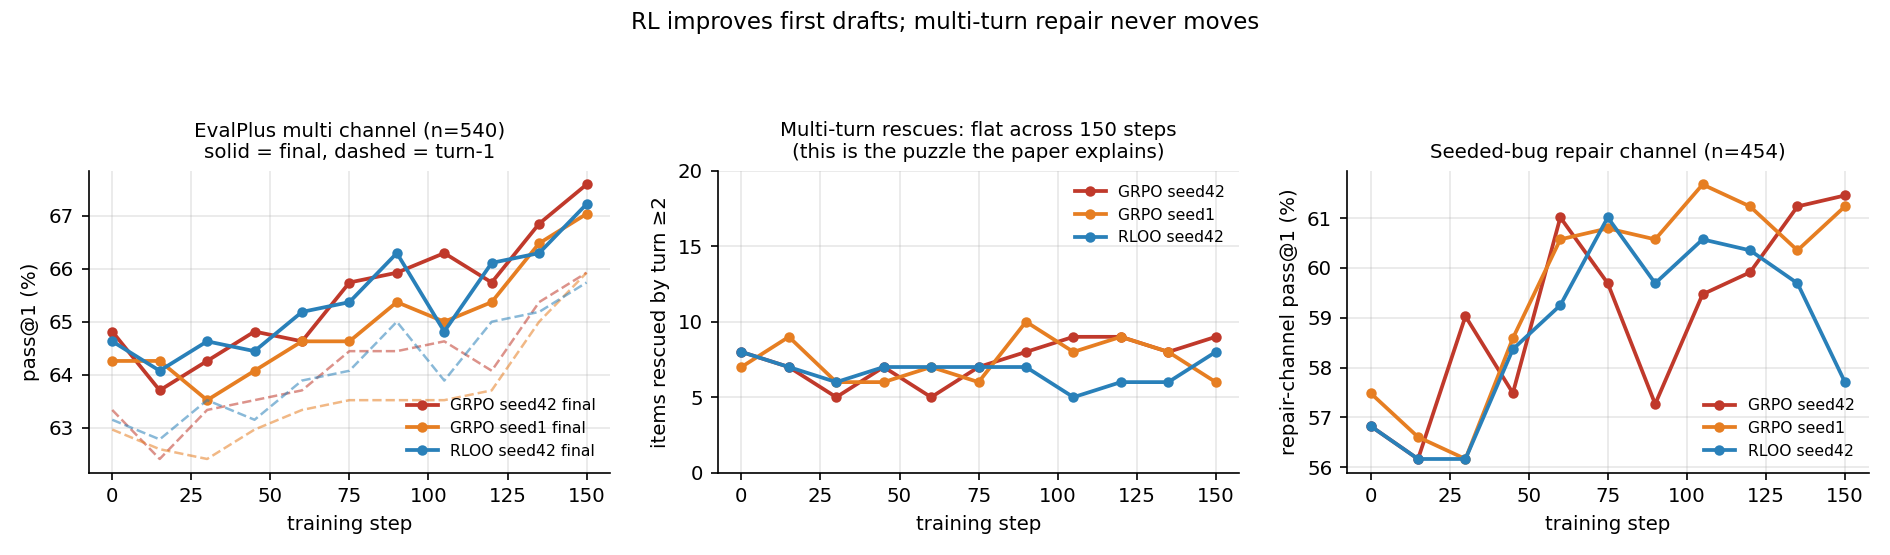
\includegraphics[width=\linewidth]{fig4_training_curves.png}
\caption{Left: pass@1 rises over 150 steps on all three runs, driven by first drafts (dashed)
rather than final answers. \textbf{Centre: the count of items rescued by turn 2 or later never
moves} --- 6--9 out of 540 from step 0 to step 150, across two algorithms and two seeds. Right:
the seeded-bug repair channel does improve, confirming the model is learning something about
fixing code; it simply never does so \emph{across turns}. \S\ref{sec:rl} shows the tool was
never successfully called in any of these runs.}
\label{fig:training_curves}
\end{figure}

\subsection{Result tables referenced from \S\ref{sec:results}}
\label{app:tables}

\begin{center}
\small
\captionof{table}{BFCL v4, first HTTP request per case. Intent columns are measured only where the parse failed.}\label{tab:bfclfunnel}
\setlength{\tabcolsep}{3.5pt}\begin{tabular}{@{}llllllll@{}}
\toprule
Arm & cases & HTTP err & first parsed & unparsed & tight & strong & weak \\
\midrule
\texttt{hermes} (documented) & 200 & 0 & \textbf{0} & 200 & 166 & 169 & 187 \\
\texttt{qwen2\_5\_coder} (repaired) & 200 & 0 & \textbf{196} & 4 & 0 & 1 & 2 \\
\bottomrule
\end{tabular}
\end{center}
\begin{center}
\small
\captionof{table}{$\tau$-bench \texttt{retail}, all 115 tasks paired across arms (none dropped).}\label{tab:tau}
\begin{tabular}{@{}lrr@{}}
\toprule
 & documented & repaired \\
\midrule
assistant turns & 1389 & 1971 \\
server-parsed calls & \textbf{0} & \textbf{636} \\
emitted but unparsed & \textbf{789} & 6 \\
tool executions / observations returned & \textbf{0} & \textbf{636} \\
\midrule
tasks entering the tool loop at all & \textbf{0} & \textbf{103} \\
tasks solved & 7 & 10 \\
\bottomrule
\end{tabular}
\end{center}
\begin{center}
\small
\captionof{table}{Same probe, items and criterion under a \emph{matched} envelope.}\label{tab:counterfactual}
\begin{tabular}{@{}lll@{}}
\toprule
Size & server-parsed & \textbf{silent fraction (tight, unparsed)} \\
\midrule
Qwen3-0.6B & 86 & \textbf{1} \\
Qwen3-1.7B & 44 & \textbf{1} \\
Qwen3-4B & 70 & \textbf{2} \\
Qwen3-8B & 97 & \textbf{0} \\
\midrule
Qwen2.5-Coder 1.5B--32B (mismatched) & 0 at every size & \textbf{0 $\to$ 4 $\to$ 21 $\to$ 36 $\to$ 80} \\
\bottomrule
\end{tabular}
\end{center}
\begin{center}
\small
\captionof{table}{Qwen2.5-Instruct under the identical mismatched configuration, with both ladders' task outcomes measured on a working executor.}\label{tab:instruct}\label{tab:turn1}
\setlength{\tabcolsep}{3.5pt}\begin{tabular}{@{}llll|ll|lll@{}}
\toprule
& \multicolumn{3}{c|}{Instruct, emitted} & \multicolumn{2}{c|}{Coder} & \multicolumn{3}{c}{Instruct} \\
Size & parsed & \textbf{tight} & weak & parsed & turn-1 = final & turn-1 & final & \textbf{rescued} \\
\midrule
1.5B & 1 & 0 & 7 & 0 & 31 & 13 & 13 & \textbf{0} \\
3B & 11 & 56 & 2 & 0 & 37 & 14 & 17 & \textbf{+3} \\
7B & 63 & 21 & 0 & 0 & 53 & 34 & 40 & \textbf{+6} \\
14B & 77 & 19 & 0 & 0 & 53 & 38 & 52 & \textbf{+14} \\
\textbf{32B} & \textbf{88} & 8 & 0 & 0 & 68 & 42 & 65 & \textbf{+23} \\
\bottomrule
\end{tabular}
\end{center}
\begin{center}
\small
\captionof{table}{Llama-3.1-8B arms, paired on the same 100 items.}\label{tab:llama_arms}
\begin{tabular}{@{}llllll@{}}
\toprule
Arm & Calls issued & Wrong-tool & Executed & Turn-1 & Final \\
\midrule
terse (parser only) & 97 & 23 & 74 & 34 & 49 \\
+ official template & 95 & 22 & 73 & 33 & 44 \\
+ official template \textbf{+ \texttt{strict}} & 98 & \textbf{0} & \textbf{97} & \textbf{46} & \textbf{61} \\
ReAct (reference) & 98 & 0 & 97 & \textbf{61} & 80 \\
\bottomrule
\end{tabular}
\end{center}
\begin{center}
\small
\captionof{table}{Decomposing the ReAct--FC gap on Llama, paired McNemar.}\label{tab:decomposition}
\begin{tabular}{@{}llll@{}}
\toprule
Comparison & b/c & \emph{p} & Attributable to \\
\midrule
terse-FC $\to$ strict-FC (49 $\to$ 61) & 15/3 & \textbf{0.0075} & \textbf{interface repair, +12} \\
strict-FC $\to$ ReAct (61 $\to$ 80) & 27/8 & \textbf{0.0019} & \textbf{protocol, +19} \\
terse-FC $\to$ ReAct (49 $\to$ 80) & 38/7 & 3.1e-06 & both, +31 \\
\bottomrule
\end{tabular}
\end{center}
\begin{center}
\small
\captionof{table}{Repair loop on Qwen2.5-Coder-7B, \texttt{tool\_choice: auto} fixed, changing only the adapter.}\label{tab:repair}
\begin{tabular}{@{}lllllll@{}}
\toprule
Arm & Parsed & Mean turns & $\geq$2 turns & Turn-1 & Final & Rescued \\
\midrule
ReAct & 95 & 1.92 & 40 & 57 & \textbf{74} & 17 \\
FC + hermes & \textbf{0} & 0.96 & \textbf{0} & 53 & 53 & \textbf{0} \\
FC + dedicated adapter & \textbf{84} & 1.82 & \textbf{37} & 53 & \textbf{62} & \textbf{9} \\
\bottomrule
\end{tabular}
\end{center}
\begin{center}
\small
\captionof{table}{RL training rollouts, matched in model, data, hyper-parameters, seed and prompt strength.}\label{tab:training}
\begin{tabular}{@{}lllll@{}}
\toprule
Arm & Steps & \texttt{num\_turns/mean} & Tool time & Tool calls / rollout \\
\midrule
FC (\texttt{tool\_agent} + hermes) & 10 & \textbf{2.000} (constant) & \textbf{0.00 s} & \textbf{0.000} \\
ReAct (\texttt{react\_agent}) & 3 & 5.883 & 12.21 s & \textbf{2.052} \\
\bottomrule
\end{tabular}
\end{center}

\subsection{Offline re-parse matrix and failure-layer decomposition}
\label{app:reparse}

To exclude ``your extractor is simply better than \texttt{hermes}'', we re-parsed the
\emph{same stored bytes} under four rules (\texttt{analysis/reparse\_matrix.py}, no GPU).

\begin{center}
\small
\captionof{table}{The same bytes, re-parsed offline under four rules. Where the server already parsed a call, \texttt{content} is empty and offline replay has nothing to read; those cells are N/A rather than zero. The gap is a parser mismatch, not a claim that no parser could have read the output.}\label{tab:reparse}
\begin{tabular}{@{}llllll@{}}
\toprule
Arm (server-parsed = 0) & server & hermes replay & \texttt{<tools>} replay & bare JSON & tight \\
\midrule
Qwen-1.5B & 0 & 0 & 0 & 0 & 0 \\
Qwen-3B & 0 & 0 & 0 & 5 & 4 \\
Qwen-7B & 0 & 0 & 0 & 22 & 21 \\
Qwen-14B & 0 & 0 & 0 & 42 & 36 \\
Qwen-32B & 0 & \textbf{0} & 0 & \textbf{100} & \textbf{80} \\
\bottomrule
\end{tabular}
\end{center}

The \texttt{hermes} column is zero at every scale: the model never produces that format. The
bare-JSON and tight columns are not: the calls exist, and their difference from the server
column is precisely what the format mismatch removes. For arms where the server \emph{did}
parse, offline content-only re-parsing is \textbf{undefined, not zero} --- a successful parse
moves the call into \texttt{tool\_calls} and leaves \texttt{content} empty.

Replaying vLLM~0.27.1's \texttt{hermes} extractor line for line over the stored bytes
(\texttt{analysis/failure\_layer.py}) separates the layer at which each item is lost: no
\texttt{<tool\_call>} envelope at all; envelope present but the JSON payload malformed; payload
well-formed and rejected only because \texttt{json.loads} does not tolerate trailing text in the
capture; or a genuine parser loss, meaning the replay succeeds where the server did not.

\begin{center}
\small
\captionof{table}{Where the unparsed items are lost. Coder fails entirely at the envelope; Instruct reaches the envelope and fails at the payload. \textbf{Genuine parser loss is zero in every arm} --- and across all 4254 de-duplicated first turns in the archive.}\label{tab:layer}
\begin{tabular}{@{}lllll@{}}
\toprule
Arm & no envelope & payload malformed & strictness only & \textbf{parser loss} \\
\midrule
Coder 1.5B--32B (all sizes) & 100 & 0 & 0 & \textbf{0} \\
Instruct 1.5B & 93 & 6 & 0 & \textbf{0} \\
Instruct 3B & 22 & 41 & 26 & \textbf{0} \\
Instruct 7B & 3 & 33 & 1 & \textbf{0} \\
Instruct 14B & 13 & 6 & 4 & \textbf{0} \\
Instruct 32B & 1 & 9 & 2 & \textbf{0} \\
\bottomrule
\end{tabular}
\end{center}

The two ladders fail at different layers: Coder emits a well-formed bare call and never the
envelope, so \texttt{hermes} not seeing it is \emph{correct behaviour}; Instruct emits the
envelope and then breaks the JSON, almost always by embedding Python whose docstring quotes or
raw newlines are left unescaped inside the \texttt{code} string. And \textbf{in no arm --- across
the whole archive --- did the server fail to parse a call that its own extractor would have
accepted.} ``Censoring'' throughout this paper therefore means \emph{the attempt never reaches
the parser in a form it is defined to accept}, not \emph{the parser discards valid calls}.

\subsection{BFCL: gating and the full reproduction record}
\label{app:bfcl}

Each arm passes a two-case end-to-end smoke test before its full run, and a run is rejected
unless the result count, the score file's \texttt{total\_count} and the number of distinct case
ids in the recording proxy all agree at 200 with zero HTTP errors. Both arms run at \texttt{max\_model\_len = 16384}, \texttt{temperature = 0} and inference seed
0, on cases drawn at manifest seed 20260901. Registration of BFCL's OpenAI
handler happens in memory at import time, so \texttt{bfcl\_eval}'s own files are left
byte-identical; a recording proxy sits between benchmark and server and logs every request.

We ran the pair twice. The \texttt{hermes} arm is identical across runs in every column: 0/200
parsed, 166 tight, 480 requests, 0 errors. The repaired arm moves by one case between runs ---
\textbf{197 versus 196} first parsed, \textbf{99 versus 98} executed --- while success is 19 in
both. Greedy decoding does not make vLLM bitwise deterministic across differing batch
compositions, and this arm runs eight threads through a multi-turn executor, so we report its
intermediate funnel columns as $\pm1$ rather than exact.

\begin{center}
\small
\captionof{table}{BFCL \texttt{multi\_turn\_base}, n = 100, joined to the HTTP trace by case id.}\label{tab:bfcl5}
\begin{tabular}{@{}lllllll@{}}
\toprule
Arm & tight (unparsed) & first parsed & any parsed & executed & \textbf{success} & rescued \\
\midrule
\texttt{hermes} & 69 & 0 & 0 & 0 & \textbf{0} & 0 \\
\texttt{qwen2\_5\_coder} & 0 & 97 & 98 & 98 & \textbf{19} & 0 \\
\bottomrule
\end{tabular}
\end{center}

\begin{center}
\small
\captionof{table}{Two quantified failure layers; the full four-family table is Table~\ref{tab:taxonomy_full}.}\label{tab:taxonomy}
\begin{tabular}{@{}p{.14\linewidth}p{.10\linewidth}p{.25\linewidth}p{.22\linewidth}p{\dimexpr.29\linewidth-8\tabcolsep\relax}@{}}
\toprule
Family & Layer & Symptom & Detectable in advance? & Remedy \\
\midrule
Qwen2.5-Coder & parser & emits a fenced JSON block, not \texttt{<tool\_call>}
  & $\times$ template check \textbf{false-positives} & dedicated adapter \\
Llama-3.1-8B & schema & calls the \emph{task function} as a tool (23\%)
  & $\times$ requires argument inspection & \texttt{strict: true} \\
\bottomrule
\end{tabular}
\end{center}

\subsection{The full four-family taxonomy}
\label{app:taxonomy}

\begin{center}
\small
\captionof{table}{Four families, four layers. Only Mistral's failure announces itself.}\label{tab:taxonomy_full}
\begin{tabular}{@{}p{.14\linewidth}p{.10\linewidth}p{.25\linewidth}p{.22\linewidth}p{\dimexpr.29\linewidth-8\tabcolsep\relax}@{}}
\toprule
Family & Layer & Symptom & Detectable in advance? & Remedy \\
\midrule
DeepSeek-Coder & template & chat template never injects tools
  & $\checkmark$ template inspection & none \\
Qwen2.5-Coder & parser & emits a fenced JSON block, not \texttt{<tool\_call>}
  & $\times$ template check \textbf{false-positives} & dedicated adapter \\
Llama-3.1-8B & schema & calls the \emph{task function} as a tool (23\%)
  & $\times$ requires argument inspection & \texttt{strict: true} \\
Mistral-7B-v0.3 & token & repeats \texttt{[TOOL\_CALLS]} $\to$ HTTP 400
  & $\sim$ errors, but only sometimes & \textbf{none found} \\
\bottomrule
\end{tabular}
\end{center}

\begin{figure}[htbp]
\centering
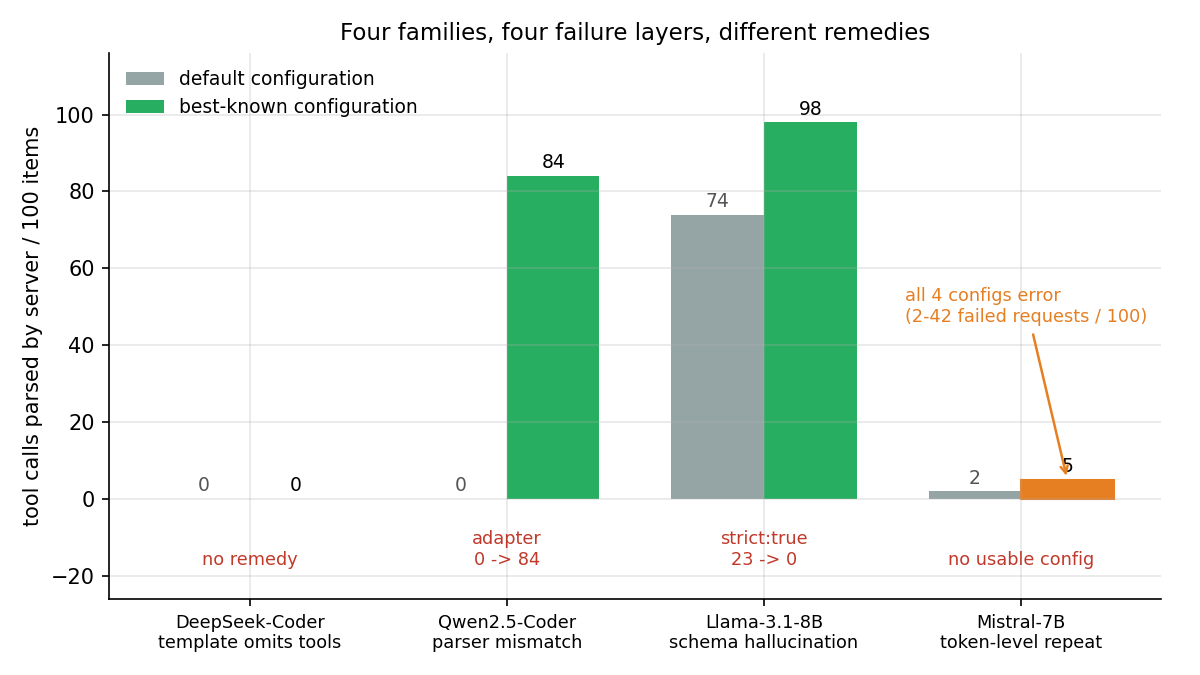
\includegraphics[width=\linewidth]{fig2_family_taxonomy.png}
\caption{The same four failures, quantified. Grey is the configuration a reader arrives at by
following the documentation; green is the best configuration we found. Mistral never produces an
error-free run under any of four configurations, so its bars are not comparable with the others
and are drawn in orange.}
\label{fig:taxonomy}
\end{figure}

\begin{figure}[htbp]
\centering

\includegraphics[width=0.72\linewidth]{fig1_intent_parse_gap.png}
\caption{Within-family observation under the mismatched interface. Across the five
Qwen2.5-Coder checkpoints, the server parses zero calls while tight-classified emissions
rise to 80/100 at 32B (approximately 72 after calibration with tight-stratum precision
0.900, assuming transfer across sizes; Appendix~\ref{app:humanval}). Same data as
Table~\ref{tab:scale}.}
\label{fig:gap}
\end{figure}

\subsection{Main table under unified configuration}
\label{sec:maintable_full}

\begin{center}
\small
\setlength{\tabcolsep}{4pt}
\captionof{table}{All arms genuinely at \texttt{max\_tokens}=2048, one shared 100-item set, \texttt{temperature}=0. Mistral has no admissible FC arm: all four configurations produce request errors, so no pass rate and no \emph{p}-value are computed.}\label{tab:main}
\setlength{\tabcolsep}{3.5pt}\begin{tabular}{@{}llllllll@{}}
\toprule
Model & \multicolumn{2}{c}{ReAct} & \multicolumn{2}{c}{FC} & b/c & \emph{p} & FC arm \\
\cmidrule(lr){2-3}\cmidrule(lr){4-5}
 & turn-1 & final & turn-1 & final & & & \\
\midrule
Llama-3.1-8B & 61 & \textbf{80} & 46 & 61 & 27/8 & \textbf{0.0019} & official tmpl.\ + \texttt{strict} \\
Qwen2.5-Coder-7B & 57 & \textbf{74} & 53 & 62 & 17/5 & \textbf{0.0169} & dedicated adapter \\
Mistral-7B-v0.3 & 26 & 33 & N/A & N/A & N/A & N/A & --- \\
\bottomrule
\end{tabular}
\end{center}

\subsection{The four Llama controls, tabulated}

\begin{center}
\small
\captionof{table}{Four single-variable controls on Llama-3.1-8B's 23\% wrong-tool rate. The first three rejected their alternative explanations and pointed at the model; the fourth found the actual cause and withdrew that conclusion.}\label{tab:controls}
\begin{tabular}{@{}p{.27\linewidth}p{.21\linewidth}p{.27\linewidth}p{\dimexpr.25\linewidth-6\tabcolsep\relax}@{}}
\toprule
Alternative explanation & Control & Empty-argument rate & Verdict \\
\midrule
schema lacks a parameter description & rich vs terse & 23 $\to$ 22 (\emph{p}=1.000) & rejected \\
ReAct merely adds a reasoning step & FC + Thought scaffold & 23 $\to$ \textbf{59} (\emph{p}\textless0.001, \textbf{worse}) & rejected \\
server not configured per documentation & + official chat template & 23 $\to$ 22 (1/0 discordance, \emph{p}=1.000) & rejected \\
\textbf{schema constraint not enabled} & \textbf{+ \texttt{strict: true} on official template} & \textbf{22 $\to$ 0 (22/0, \emph{p}=4.77$\times10^{-7}$)} & \textbf{accepted} \\
\bottomrule
\end{tabular}
\end{center}

\subsection{Conditioning on a successful parse, and access vs.\ use of feedback}
\label{app:conditioned}

\begin{center}
\small
\captionof{table}{Conditioning on items where both protocols parsed successfully. The residual protocol gap holds on Llama and does not reach significance on Qwen --- the honest reading is one family out of two, not a general law.}\label{tab:conditioned}
\begin{tabular}{@{}llllll@{}}
\toprule
Family & Items both parsed & ReAct & FC & b/c & \emph{p} \\
\midrule
Qwen2.5-Coder-7B & 83 & 63 & 56 & 11/4 & \textbf{0.119 (n.s.)} \\
Llama-3.1-8B & 96 & 78 & 60 & 25/7 & \textbf{0.0021} \\
\bottomrule
\end{tabular}
\end{center}

\begin{center}
\small
\captionof{table}{Repair success given that feedback was actually received. Conditioned this way the two protocols are much closer, which locates the gap in \emph{how often feedback arrives} rather than in what the model does with it. On Qwen this difference is within the non-significant band above, so we state it as an observation, not a result.}\label{tab:given_feedback}
\begin{tabular}{@{}llll@{}}
\toprule
Arm & Reached turn $\geq$2 & Rescued & Repair success given feedback \\
\midrule
ReAct & 40 & 17 & \textbf{42\%} \\
FC + adapter & 37 & 9 & \textbf{24\%} \\
FC + hermes & \textbf{0} & \textbf{0} & undefined \\
\bottomrule
\end{tabular}
\end{center}

\textbf{Adapters are not a universal switch.} The same adapter recovers 84/100 at 7B and
\textbf{1/100 at 3B}: the 3B checkpoint ignores the \texttt{<tools>} few-shot entirely (zero
\texttt{<tools>} tags in 100 items, 99 direct code) while still solving the task at a comparable
rate (final 53). Adapter effectiveness is non-monotonic in scale, reinforcing the per-checkpoint
claim of \S\ref{sec:families}. The dedicated solution also changes parser, chat template and
few-shot simultaneously; we additionally rewrote the template's few-shot examples, which
originally invoked \texttt{get\_weather} --- a tool absent from our schema, which would have
induced calls to a non-existent tool and inflated both initiation and empty-argument counts.
Original and modified hashes are recorded.

\subsection{Pressure on a broken interface makes things worse}
\label{sec:pressure}

Two independent controls point the same way. Adding a reasoning scaffold to FC raised role
confusion from 23 to \textbf{59} (\S\ref{sec:llama}). Replacing the optional tool instruction
with a mandatory one on Qwen2.5-Coder-1.5B moved parser-accepted calls not at all --- still
0/100 --- while final pass fell from \textbf{31 to 15} and unparsable outputs rose from
${\sim}0$ to 46/100. Neither intervention touches the interface, and both make the observable
outcome worse. \textbf{When an agent appears reluctant to use tools, strengthening the
instruction is the cheapest thing to try and the most likely to mislead} --- it can degrade task
performance while leaving the tool-call count at zero, which looks like a model that is both
unwilling \emph{and} incapable.

\begin{center}
\small
\captionof{table}{Probe replication on the 1.5B model actually being trained, same mandatory prompt (n=100). Not one output names \texttt{run\_tests}, so at this scale the missing calls are not a parser mismatch --- there was nothing well-formed to censor.}\label{tab:probe_categories}
\begin{tabular}{@{}lll@{}}
\toprule
Category & n & \% \\
\midrule
wrong name, \texttt{arguments} carry complete code & \textbf{0} & 0\% \\
wrong name, \texttt{arguments} are the task function's parameters & \textbf{36} & 69\% \\
wrong name, executable code present elsewhere in the body & 16 & 31\% \\
\bottomrule
\end{tabular}
\end{center}

\begin{center}
\small
\captionof{table}{Increasing pressure on the 1.5B model. Stronger instruction and few-shot examples raise the number of recoverable code payloads but never produce a call that names the tool.}\label{tab:pressure}
\begin{tabular}{@{}llll@{}}
\toprule
& recoverable calls & \textbf{naming \texttt{run\_tests}} & final pass \\
\midrule
mandatory prompt (baseline) & 52 & \textbf{0} & 15 \\
+ role-disambiguation few-shot & \textbf{64} & \textbf{0} & \textbf{13} \\
\bottomrule
\end{tabular}
\end{center}

\subsection{Formal 7B checkpoint curve and final-lineage audit}
\label{app:p3curve}

All checkpoint evaluations use the same 542-item multi-turn manifest, have zero request failures,
and attest the indicated native weight step. The accepted curve uses the original repaired steps
0--90 and resumed steps 120--150; the abandoned original steps 91--116 are excluded. The repeated
step-90 evaluation after resumption gave 415/426/11 rather than 415/428/13 and is retained as
test--retest evidence, not substituted into the formal curve.

\begin{center}
\small
\captionof{table}{Complete formal 7B held-out curve. Each cell is turn-1 pass / final pass / rescued after turn 1, with $n=542$.}\label{tab:p3curve}
\begin{tabular}{@{}lrr@{}}
\toprule
step & broken FC & repaired FC \\
\midrule
0   & 418 / 430 / 12 & 418 / 430 / 12 \\
30  & 418 / 430 / 12 & 418 / 429 / 11 \\
60  & 420 / 433 / 13 & 417 / 431 / 14 \\
90  & 418 / 432 / 14 & 415 / 428 / 13 \\
120 & 419 / 433 / 14 & 415 / 427 / 12 \\
150 & 418 / 430 / 12 & 415 / 427 / 12 \\
\bottomrule
\end{tabular}
\end{center}

The policies did update. The accepted logs contain all 150 steps with non-zero actor gradient
norms: 0.0120--0.0251 for broken and 0.00641--0.01599 for repaired; mean training rewards span
0.150--0.469 and 0.168--0.435, respectively. A direct checkpoint audit over all 392 LoRA tensors
(80{,}740{,}352 parameters) finds 45{,}471{,}572 values changed from broken step 120 to 150
(56.3\%, $\ell_2$ delta 0.0787) and 45{,}296{,}056 from repaired step 90 to resumed step 150
(56.1\%, $\ell_2$ delta 0.1222). These comparisons establish updates to saved LoRA weights
over the retained intervals; evaluation completion records separately attest the native weight step.

The event join also resolves the funnel's apparent gaps. Broken FC has 19{,}203 generation events,
8{,}689 tight emissions and 10 accepted/executed/observed calls. Repaired FC has 33{,}367
generation events, 17{,}608 tight emissions, and 16{,}912 accepted calls in 16{,}844 accepted
generation events. Forty generations contain multiple calls, producing exactly the 68-call surplus;
all 16{,}844 dispatches join to executions and observations by request ID and assistant turn.
Extraction records lack those identifiers; accepted-generation and dispatch counts match per
trajectory, rather than through a per-generation join. Tight and accepted are different tests:
16{,}323 events satisfy both, 1{,}285 are tight but unaccepted, and 521 are accepted but not tight.
The repository's \texttt{analysis/p3\_final\_evidence.py} verifies all evaluation and event hashes,
reconstructs the final lineage, and emits the per-file manifest; the server-side checkpoint audit is
reproducible with \texttt{analysis/p3\_checkpoint\_lora\_audit.py}.

\subsection{Historical ReAct positive control, tabulated}

\begin{figure}[htbp]
\centering
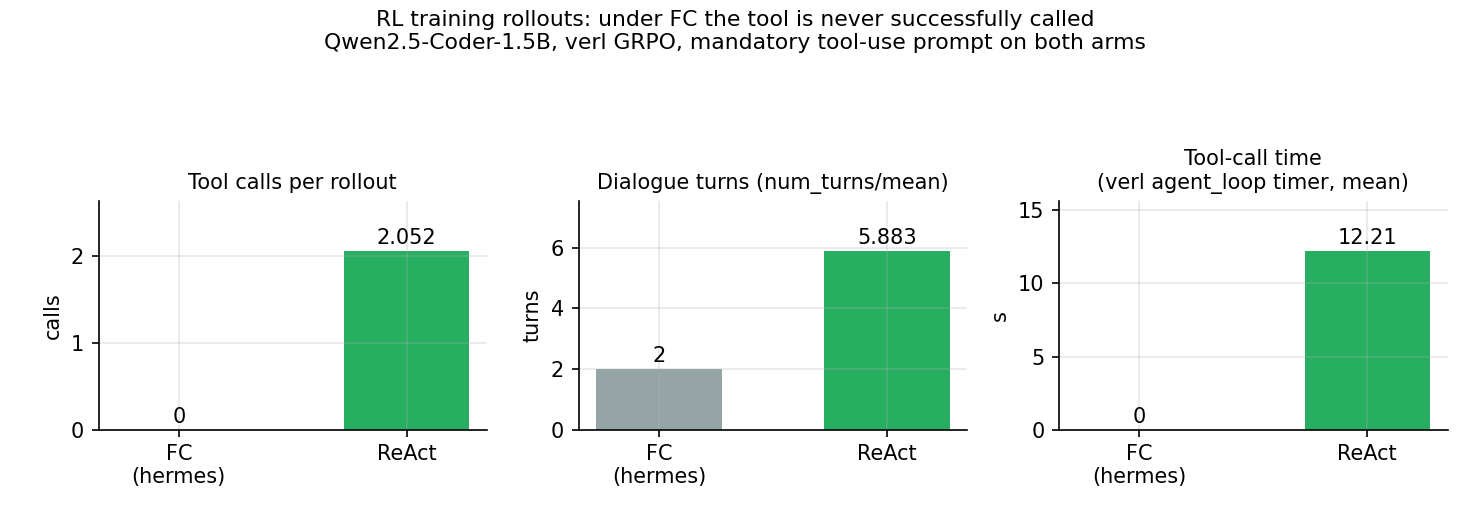
\includegraphics[width=\linewidth]{fig3_training_causal.png}
\caption{\textbf{Historical 1.5B RL diagnostic.} Under function calling the tool is never
successfully called; \texttt{num\_turns} stays pinned at its minimum of 2 and tool time is exactly
zero. Prompt strength is matched across arms (both mandatory); step counts are not (10 vs 3).
The formal 7B parser control is reported separately in Table~\ref{tab:p3formal}.}
\label{fig:train}
\end{figure}

\begin{center}
\small
\captionof{table}{Historical ReAct training with a working tool channel, 23{,}676 executed calls. Rescues by turn $\geq$2 do not move. The three historical 1.5B FC runs, in which \textbf{zero} tool calls executed, give rescue sequences $[7,9,6,6,7,6,10,8,9,8,6]$, $[8,7,6,7,7,7,7,5,6,6,8]$ and $[7,5,7,5,7,8,9,9,8,9]$. This is supporting evidence only; Table~\ref{tab:p3formal} is the single-variable control.}\label{tab:sufficiency}
\begin{tabular}{@{}lrrrr@{}}
\toprule
step & turn-1 & final & \textbf{rescued by turn $\geq$2} & repair channel \\
\midrule
0  & 359 & 367 & 8 & 263 \\
15 & 340 & 346 & \textbf{6} & 266 \\
30 & 340 & 346 & \textbf{6} & 262 \\
45 & 341 & 349 & \textbf{8} & 261 \\
60 & 341 & 347 & \textbf{6} & 274 \\
\bottomrule
\end{tabular}
\end{center}

\subsection{Sampling variance, and an inverted noise structure}
\label{sec:variance}

Llama-3.1-8B, \texttt{temperature=0.6}, n=100 $\times$ 3 seeds.

\begin{center}
\small
\captionof{table}{Sampling variance. FC seed 3 contains one rejected parallel-call request. We report its complete-denominator endpoint, and treat the two clean arms separately; an SD from two clean seeds would be too unstable to summarize variation reliably.}\label{tab:variance}
\begin{tabular}{@{}lllll@{}}
\toprule
& seed 1 & seed 2 & seed 3 & admissible \\
\midrule
ReAct turn-1 & 53 & 56 & 43 & 3/3 \\
ReAct final & 72 & 72 & 72 & 3/3 \\
FC turn-1 & 44 & 44 & 45 & --- \\
FC final & 62 & 66 & 57$^{\dagger}$ & \textbf{2 clean / 3 end-to-end} \\
\bottomrule
\end{tabular}
\end{center}

FC seed 3 contains one request error --- the model emitted parallel tool calls and vLLM returned
\emph{``This model only supports single tool-calls at once''}. The end-to-end endpoint therefore
retains that task as a failure and is 57/100; the prespecified clean-arm analysis excludes the seed
and reports [62, 66]. An SD can be computed from two clean seeds, but would be an unstable estimate,
so we do not use it to characterize sampling variation. Worst case among clean arms: ReAct's
lowest (72) versus FC's highest (66) = \textbf{+6}.

\textbf{Inverted noise structure.} ReAct's turn-1 varies widely (43--56, sd 6.8) while its final
converges; FC's turn-1 is nearly constant (44--45, sd 0.58) while its final disperses. The
mechanism is compensation in the rescue count --- 19 / 16 / \textbf{29}, largest where turn-1 was
worst --- and in all three seeds the count of ``passed at turn 1 but failed finally'' is
\textbf{0}: the repair loop is monotone. \textbf{The three identical finals are a coincidence of
totals, not identical item sets}, and sd = 0.00 must not be read as ``ReAct is perfectly
stable''.

\subsection{Multi-turn repair stabilises the total while its composition keeps moving}
\label{sec:composition}

Two independent observations show the same structure. \emph{Across sampling seeds}: ReAct's final
pass is 72 / 72 / 72 at \texttt{temperature=0.6}, yet the solved sets have pairwise Jaccard
0.71--0.80 --- 15--24 items differ. \emph{Across training steps}: between steps 15 and 30 of the
ReAct run, 85 of 542 first-turn completions changed verbatim and 6 items flipped outcome (3
gained, 3 lost), leaving turn-1 and final pass numerically identical (340 / 346 at both
checkpoints). The policy is demonstrably moving; the aggregate is not.

The common structure is that \textbf{the repair loop absorbs perturbation upstream of it}. Two
consequences follow. \emph{For measurement}, an aggregate pass rate is a \textbf{poor instrument
for detecting change in a multi-turn agent}: it is stabilised by the very mechanism under study,
and item-level set comparison detects movement the total conceals. We report both throughout, and
note that had we reported only totals we would have concluded --- twice, on two different axes ---
that nothing was happening. \emph{For deployment}, stability of the total under sampling noise is
a property practitioners want, it is contributed by the multi-turn loop rather than the base
policy, and it is invisible in single-turn evaluation. \textbf{Bound}: both observations are on
one model family and one task, the identical totals are in part coincidence, and we do not claim
the aggregate is invariant --- only that it is far less sensitive than its components.

\subsection{The training verifier: seams, audit, and planned fixes}
\label{app:verifier}

The GRPO reward is outcome-only: it extracts the last submitted program, runs the item's own
\texttt{pytest} suite in the sandbox, and returns the pass ratio (\texttt{reward\_code.py}). Three
reward-hacking routes are closed by construction --- a run in which no test executes scores 0
rather than 1, a timeout scores 0, and an item with no test string scores 0. The historical
verifier nevertheless had two seams. \emph{(i)} Its summary parser searched
\texttt{(\textbackslash d+) passed} over merged stdout/stderr and took the first match, so model
stdout could imitate pytest's summary. \emph{(ii)} \texttt{skipped} and \texttt{xfail} were not
counted in the denominator. Both were reachable in principle. We therefore audited:
across the five training logs that retain generated code there are \textbf{zero} occurrences of a
printed \texttt{``N passed''}, of \texttt{pytest.skip}/\texttt{allow\_module\_level}, or of
\texttt{sys.exit}/\texttt{os.\_exit}, and \texttt{critic/rewards/mean} oscillates in 0.46--0.73
without the step change a discovered exploit produces. The audit's own limit is that historical
full rollout text was not retained, so it covers only the fragments those logs carry. Before the
formal 7B control we anchored the regex to pytest's summary, included
\texttt{skipped}/\texttt{xfailed}/\texttt{xpassed} in the denominator, and retained every rollout
in full with a SHA-256 digest. Both P3 arms use this fixed verifier. Neither verifier path is used
for the reported held-out pass rates, which require \texttt{mode="script"}, a zero exit code and
\texttt{status=="ok"}.


\end{document}
